\documentclass{beamer}
%
% Choose how your presentation looks.
%
% For more themes, color themes and font themes, see:
% http://deic.uab.es/~iblanes/beamer_gallery/index_by_theme.html
%

\definecolor{sidegray}{RGB}{77,128,137}
\definecolor{headgray}{RGB}{72,72,72}
\definecolor{logogray}{RGB}{78,78,78}

\mode<presentation>
{
  \usetheme[hideothersubsections]{PaloAlto} %PaloAlto     % or try Darmstadt, Madrid, Warsaw, ...
  \usecolortheme{dolphin} % dolphin or try albatross, beaver, crane, ...
  \usefonttheme{serif}  % or try serif, structurebold, ...
  %\setbeamertemplate{navigation symbols}{}
  \setbeamertemplate{caption}[numbered]
  \setbeamercolor{sidebar}{bg=sidegray!90!black}
  \setbeamercolor{frametitle}{bg=sidegray!90!black}
  \setbeamercolor{logo}{bg=sidegray!50!black} 
  %\setbeamercolor{background canvas}{bg=violet}
  %\setbeamertemplate{sidebar left}[]
} 



\usepackage[spanish]{babel}
\usepackage[utf8]{inputenc}
\usepackage{tikz}

\title[Tesis de Grado de Ingeniería Electrónica]{Análisis e Implementación de algoritmos FFT para
transmisiones OFDM}
\author[Andres Dario Cassagnes]{\textit{Alumno:} Sr. Andrés Dario Cassagnes\\
\small{\textit{Director:} Dr. Ing. Ariel Lutenberg}\\
\small{\textit{Codirector:} Ing. Federico Giordano Zacchigna}}
\institute{Laboratorio de Sistemas Embebidos\\ Facultad de Ingeniría\\ Universidad de Buenos Aires}
\date{15/12/2016}
%\logo{
\includegraphics[scale=0.10]{./figures/logoFIUBA.png}}

% \makeatletter
% %\setbeamertemplate{sidebar canvas left}{}
% \setbeamertemplate{sidebar left}[sidebar theme]{%
%     \vspace*{3.5cm}
%     \vspace*{\fill}
%     %\includegraphics[width=1.25cm]{ire_logo.png}\\
%     %\includegraphics[width=1.25cm]{weiti_logo.png}\\
%     %\includegraphics[width=1.25cm]{pw_logo.png}
%     \vspace*{0.1cm}
%     \vfill
% 
% }
% \makeatother

\makeatletter
%\beamer@sidebarwidth=5 \baselineskip     %controls the height of the headline, default is 2.5
\beamer@headheight=1.5\baselineskip     %controls the height of the headline, default is 2.5 
%\setlength\beamer@sidebarwidth{2cm}   
\makeatother

\hyphenation{Im-ple-men-ta-cion}

\begin{document}

\begin{frame}
% \tikz [remember picture,overlay]
%     \node at
%         ([yshift=1.5cm]current page.south)
%         ([xshift=1cm]current page.south) 
%         %or: (current page.center)
%         {
\includegraphics[scale=0.10]{./figures/logoFIUBA.png}};
  \titlepage
\end{frame}

% Uncomment these lines for an automatically generated outline.
%\begin{frame}{Outline}
%  \tableofcontents
%\end{frame}

\section{Introducci�n}

\begin{frame}{OFDM}
  \begin{columns}[T]
    \begin{column}{.3\textwidth}
      \begin{itemize}
        \item Orthogonal Frequency Divider Multiplexing
        \item<2-> Divide la informaci�n en m�ltiples frecuencias
        \item<3-> Bandas de frecuencia solapadas
      \end{itemize}
    \end{column}
    
    \begin{column}{.7\textwidth}
      \uncover<2->{
        \alt<2>{
          \begin{center}
            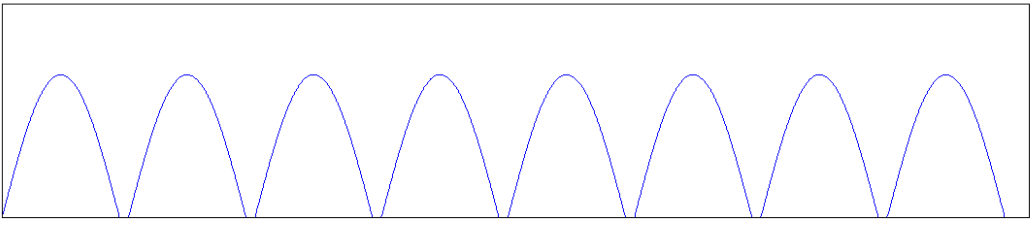
\includegraphics[scale=0.17]{./figures/freq_mux.png}
          \end{center}
        }{
        %\uncover<4->{
          \begin{center}
            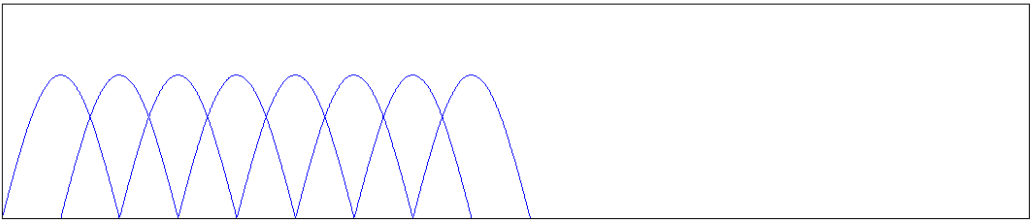
\includegraphics[scale=0.17]{./figures/freq_ort.png}
          \end{center}
        }
      }
    \end{column}
  \end{columns}
  
  \begin{itemize}
    \item<4-> Representaci�n matem�tica
  \end{itemize}
  \uncover<4->{
	  \begin{equation}
		s_{k}(t-kT) =
		%	\begin{cases}
			\sum\limits_{i=-N/2}^{N/2-1} x_{i,k} e^{j2\pi
			\left(\frac{i}{T}\right)(t-kT)}
		%	\end{cases}
		\end{equation}
	}
	
  \begin{itemize}
    \item<5-> Asumiendo que $x_{i,k}$ es constante a lo largo del per\'iodo de s\'imbolo $T$, se puede utilizar una IDFT\slash DFT para modular.
  \end{itemize}
  
%   \begin{columns}[T]
%     \begin{column}{.5\textwidth}
%       \uncover<6->{
%         \begin{center}
%           \advance\leftskip-0.2cm
%           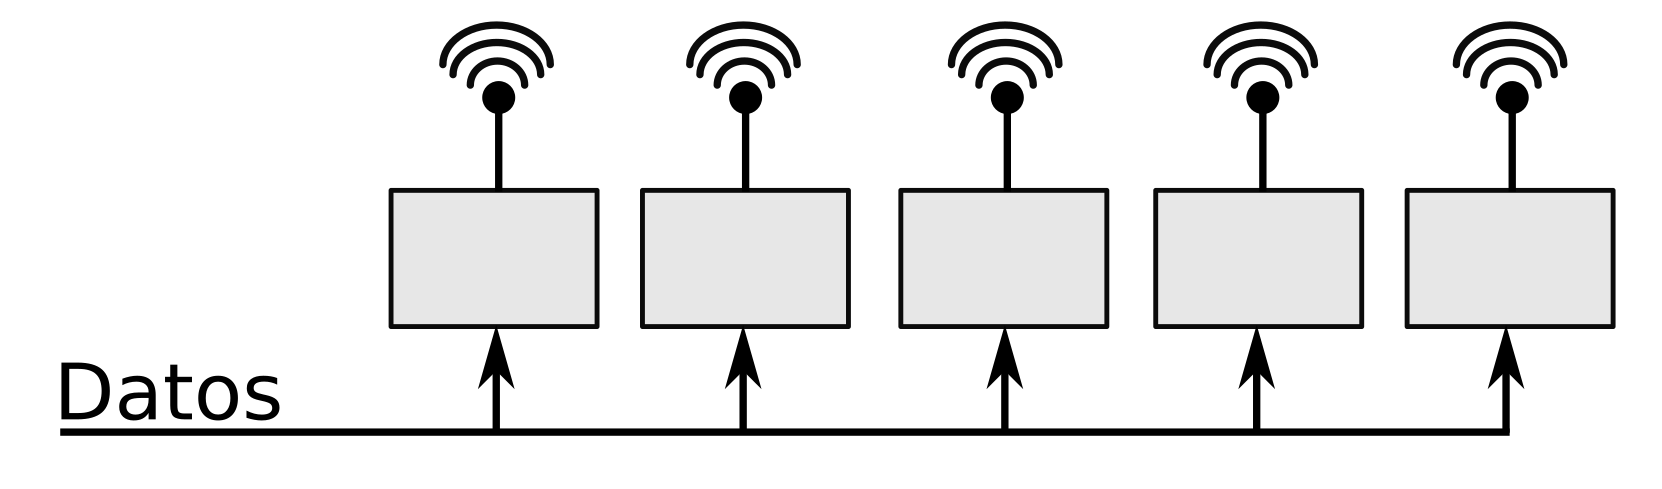
\includegraphics[scale=0.26]{./figures/hard_mod.png}
%         \end{center}
%       }
%     \end{column}
%     
%     \begin{column}{.5\textwidth}
%       \uncover<8->{
%         \begin{center}
%           \advance\leftskip-0.2cm
%           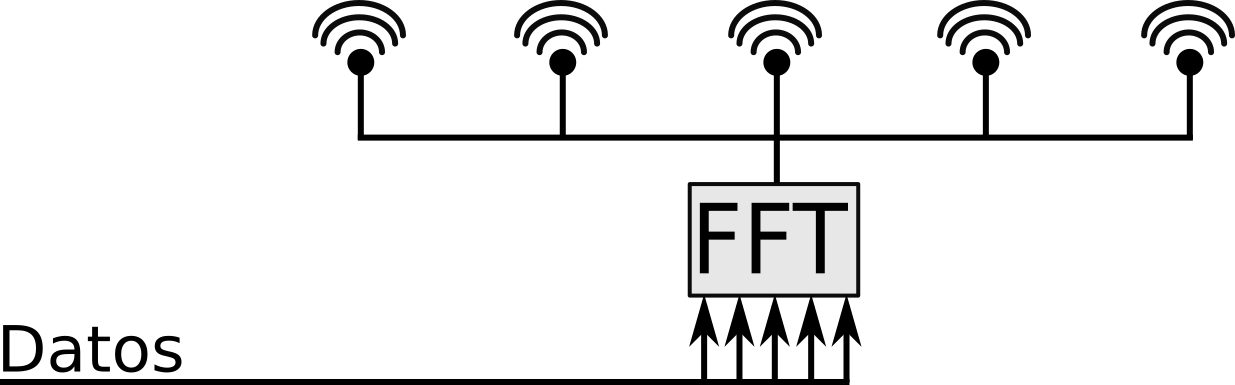
\includegraphics[scale=0.26]{./figures/soft_mod.png}
%         \end{center}
%       }
%     \end{column}
%   \end{columns}
	
  
 
\end{frame}

\begin{frame}{FFT}
  \Fontit
  \begin{itemize}
    \item<1-> Transformada r�pida de Fourier
    \item<2-> Sumas/restas y multiplicaciones
    \item<3-> Cada salida = suma y resta de todas las entradas
  \end{itemize}

  \vfill

  \uncover<3->{
    \begin{center}
      \advance\leftskip-0.2cm
      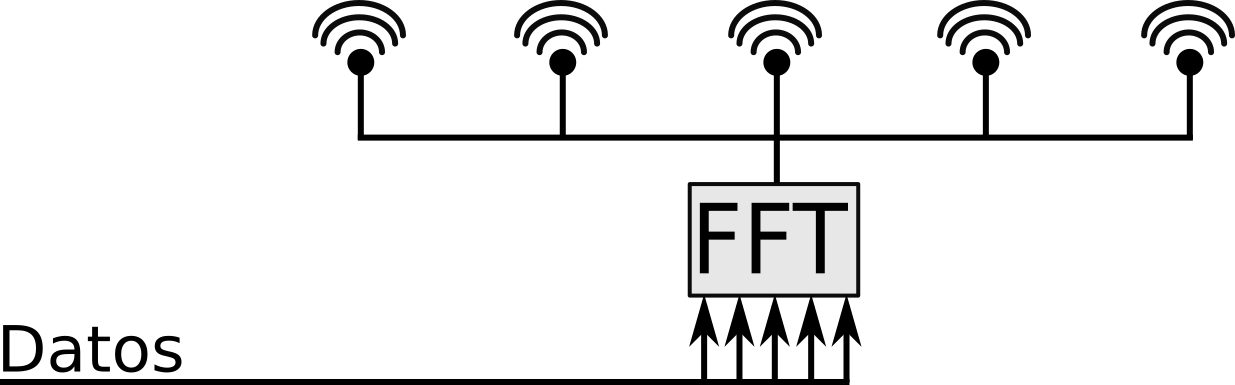
\includegraphics[scale=0.30]{./figures/soft_mod.png}
    \end{center}
  }

\end{frame}
% 
% \begin{frame}{FPGA}
% 
% \begin{columns}[T]
%   \begin{column}{.2\textwidth}
%       \uncover<2->{
%         \alt<2>{
%         \begin{center}
%           \advance\leftskip-0.2cm
%           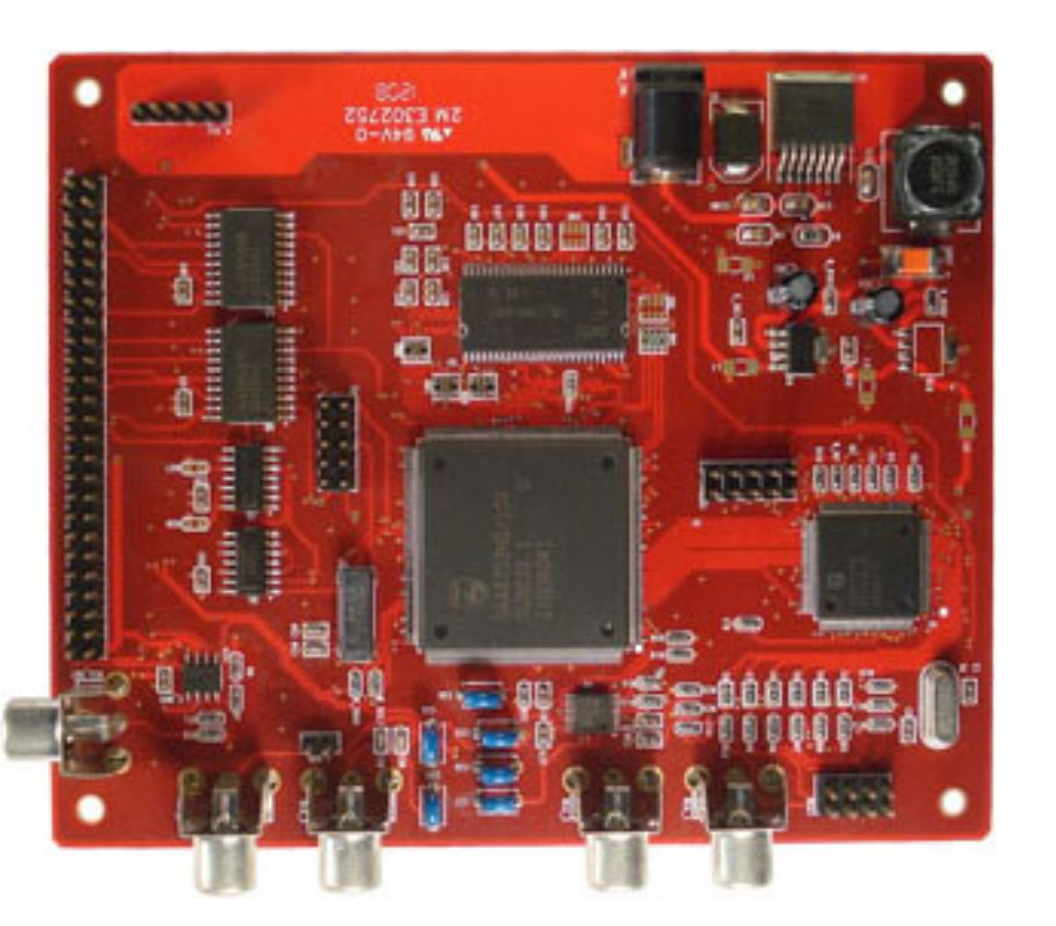
\includegraphics[scale=0.20]{./figures/circ_good.png}
%         \end{center}
%         }{
%         \begin{center}
%           \advance\leftskip-0.2cm
%           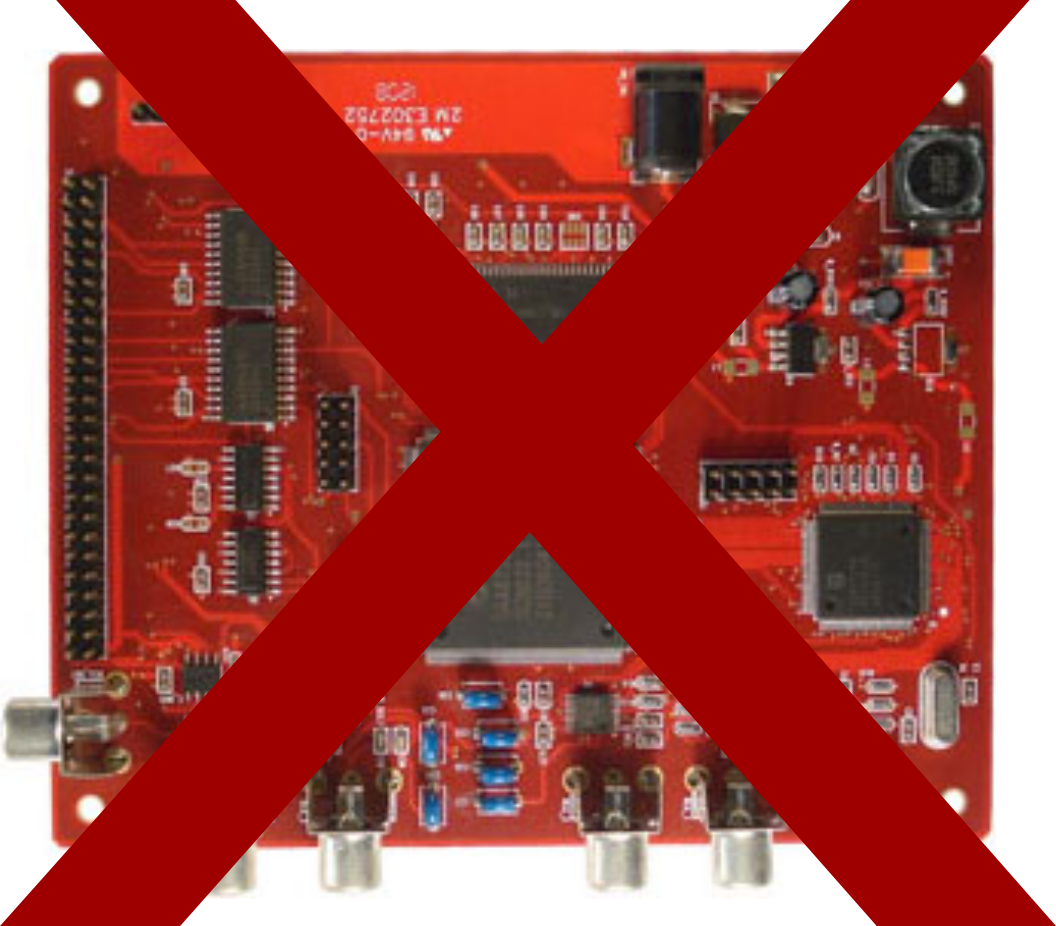
\includegraphics[scale=0.20]{./figures/circ_bad.png}
%         \end{center}
%         }
%       }
%     \end{column}
%     \begin{column}{.2\textwidth}
%       \uncover<4->{
%         \begin{center}
%           \advance\leftskip-0.2cm
%           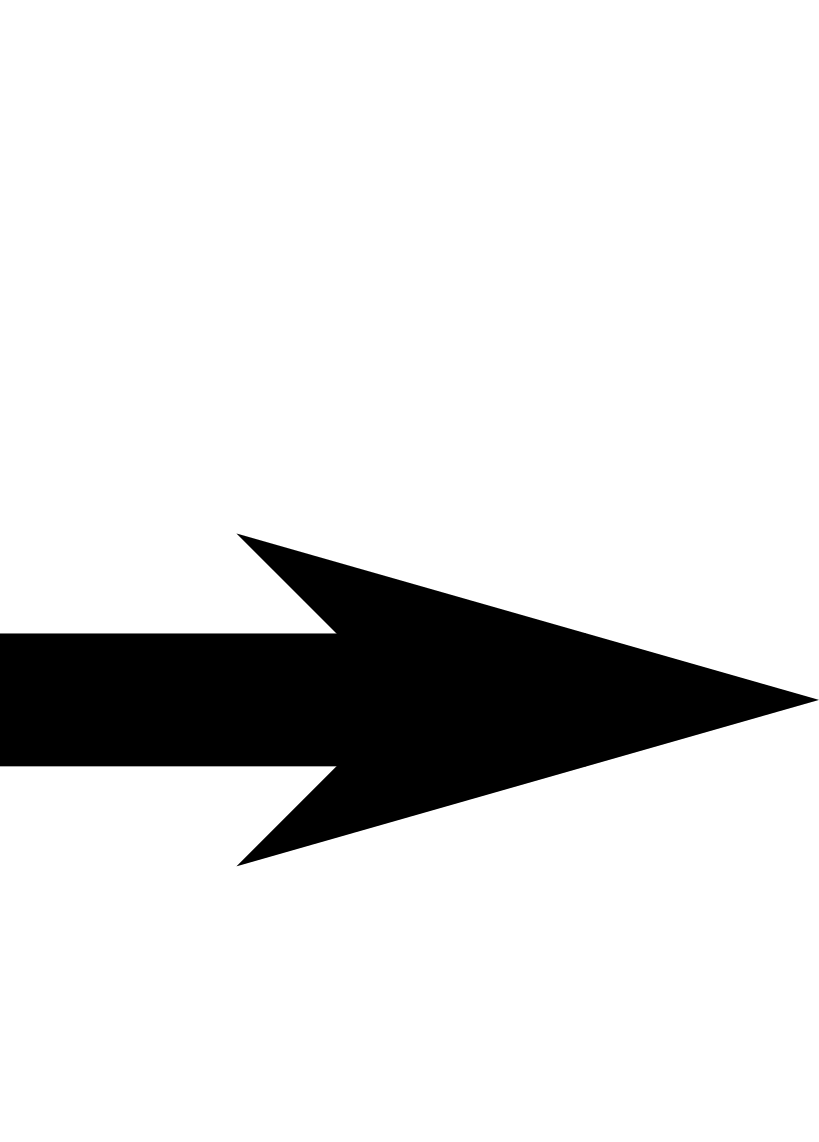
\includegraphics[scale=0.13]{./figures/flecha.png}
%         \end{center}
%        }
%     \end{column}
%     
%     \begin{column}{.2\textwidth}
%       \uncover<5->{
%         \alt<5>{
%         \begin{center}
%           \advance\leftskip-0.2cm
%           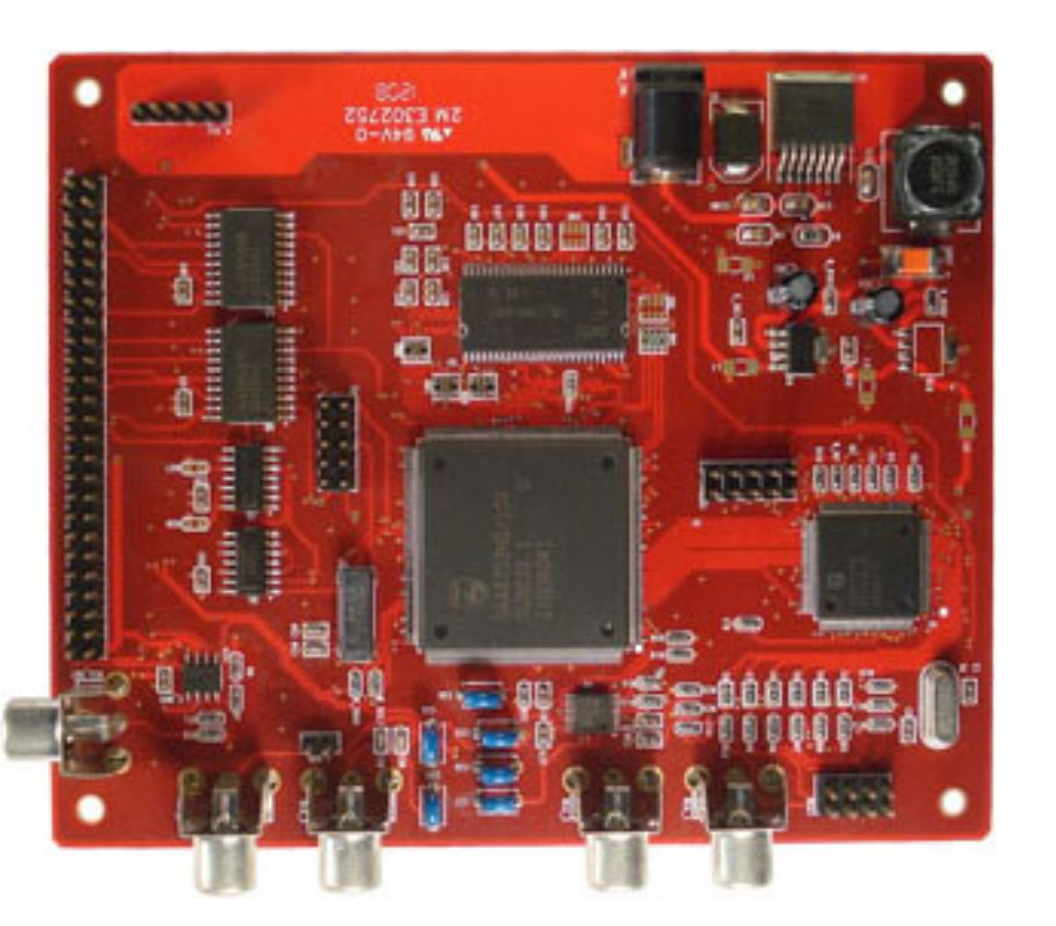
\includegraphics[scale=0.20]{./figures/circ_good.png}
%         \end{center}
%         }{
%         \begin{center}
%           \advance\leftskip-0.2cm
%           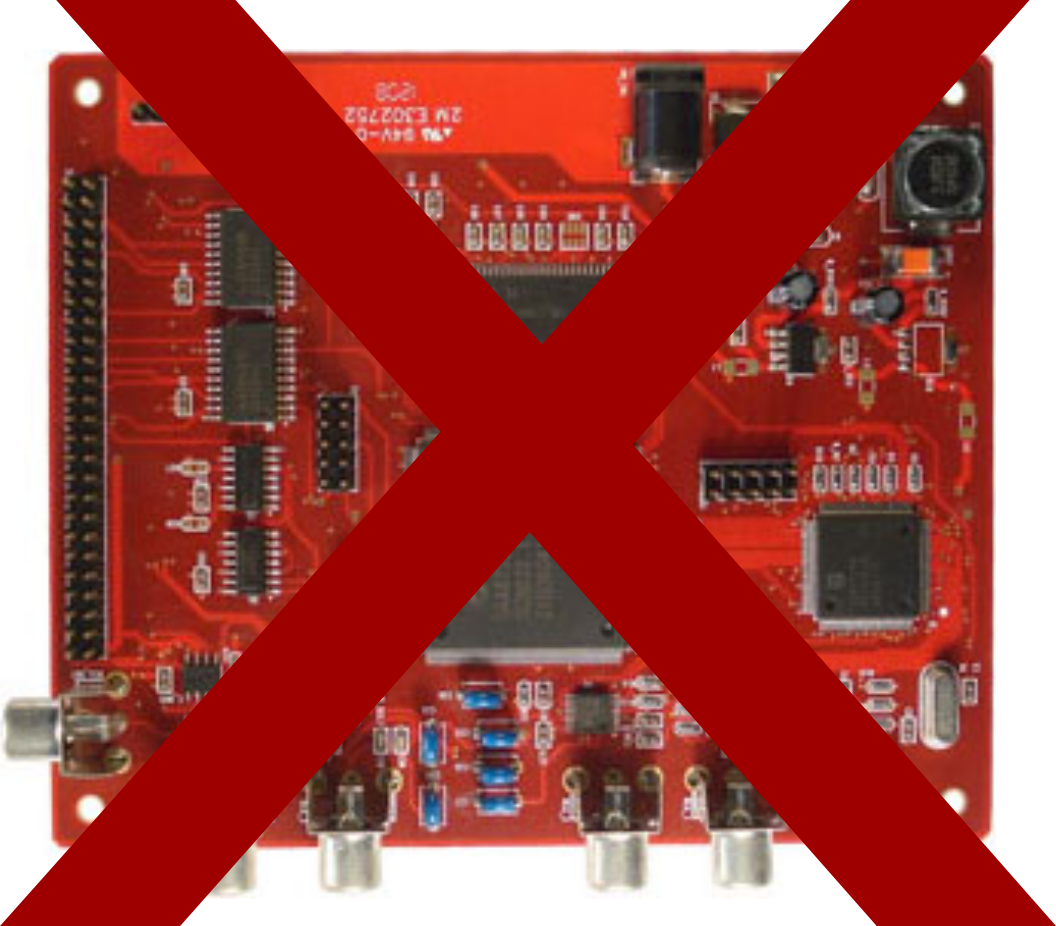
\includegraphics[scale=0.20]{./figures/circ_bad.png}
%         \end{center}
%         }
%       }
%     \end{column}
%     \begin{column}{.2\textwidth}
%       \uncover<6->{
%         \begin{center}
%           \advance\leftskip-0.2cm
%           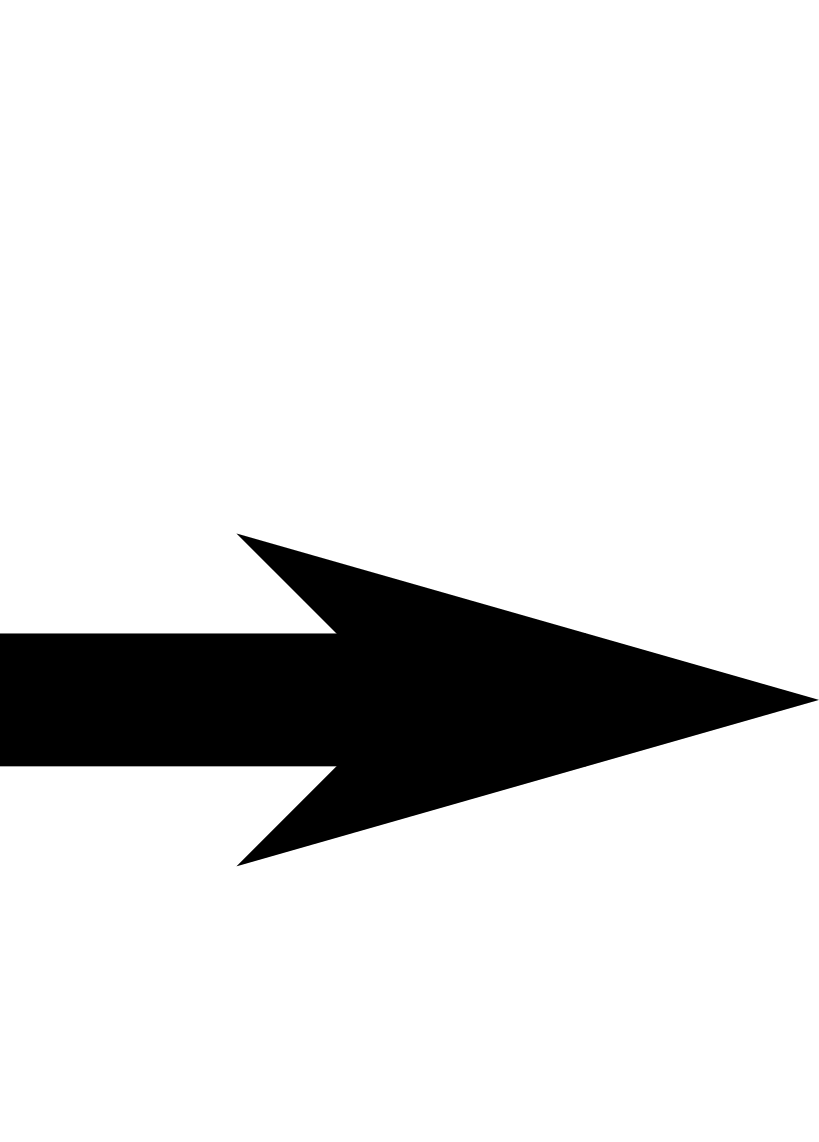
\includegraphics[scale=0.13]{./figures/flecha.png}
%         \end{center}
%        }
%     \end{column}
%     
%     \begin{column}{.2\textwidth}
%       \uncover<7->{
% %         \alt<7>{
%         \begin{center}
%           \advance\leftskip-0.2cm
%           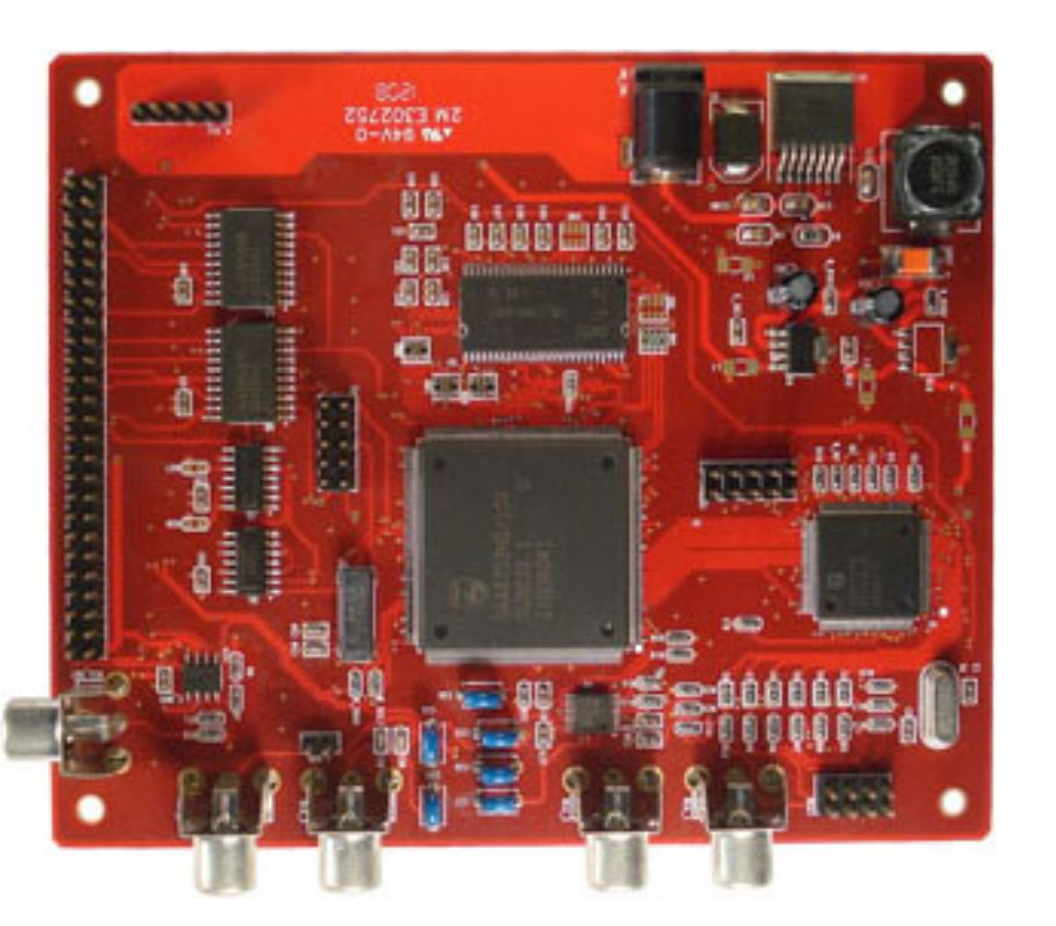
\includegraphics[scale=0.20]{./figures/circ_good.png}
%         \end{center}
% %         }{
% %         \begin{center}
% %           \advance\leftskip-0.2cm
% %           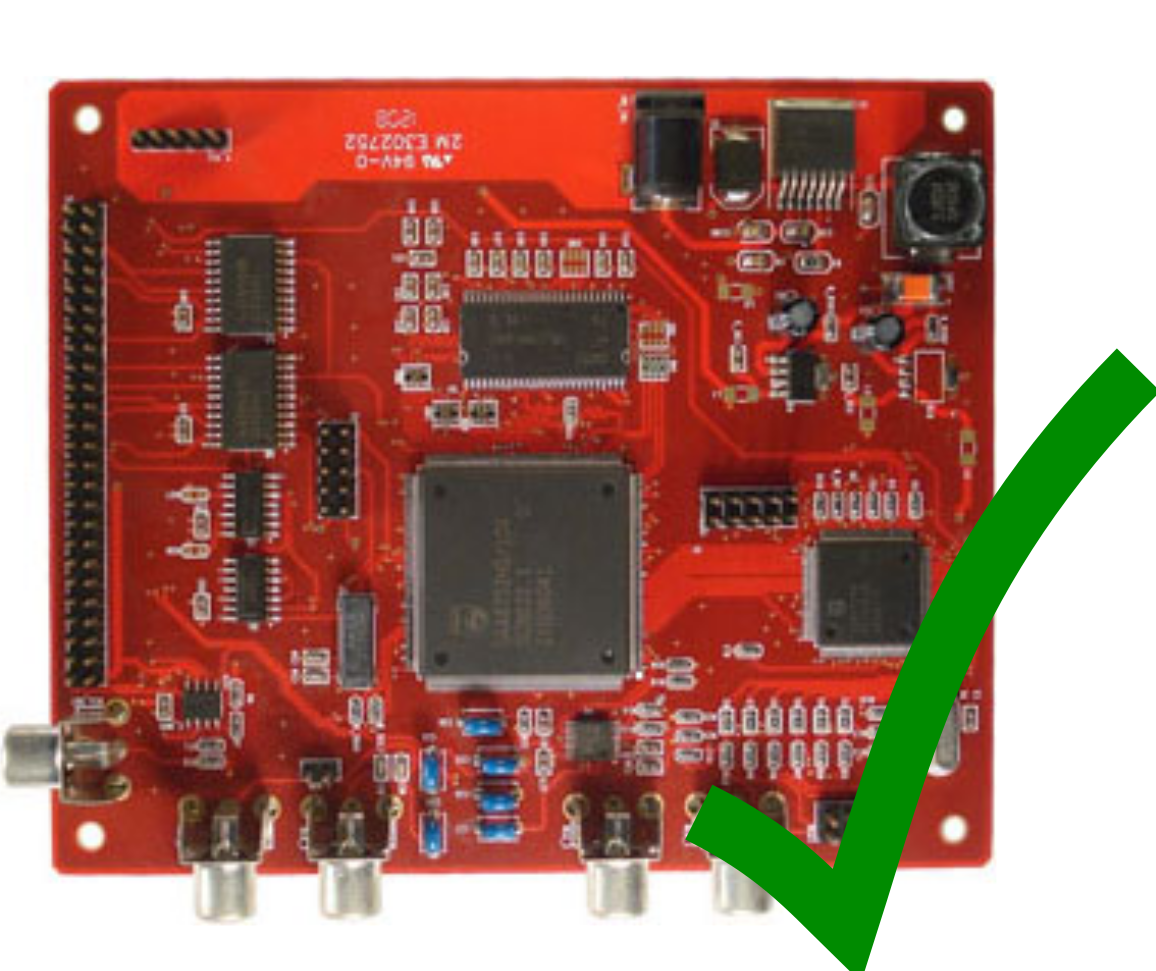
\includegraphics[scale=0.20]{./figures/circ_tick.png}
% %         \end{center}
% %         }
%       }
%     \end{column}
%     
%     
%     
%   \end{columns}
%   
%   \vfill
%   
%   \uncover<8->{
% 	  \begin{center}
% 		  \advance\leftskip-0.2cm
% 		  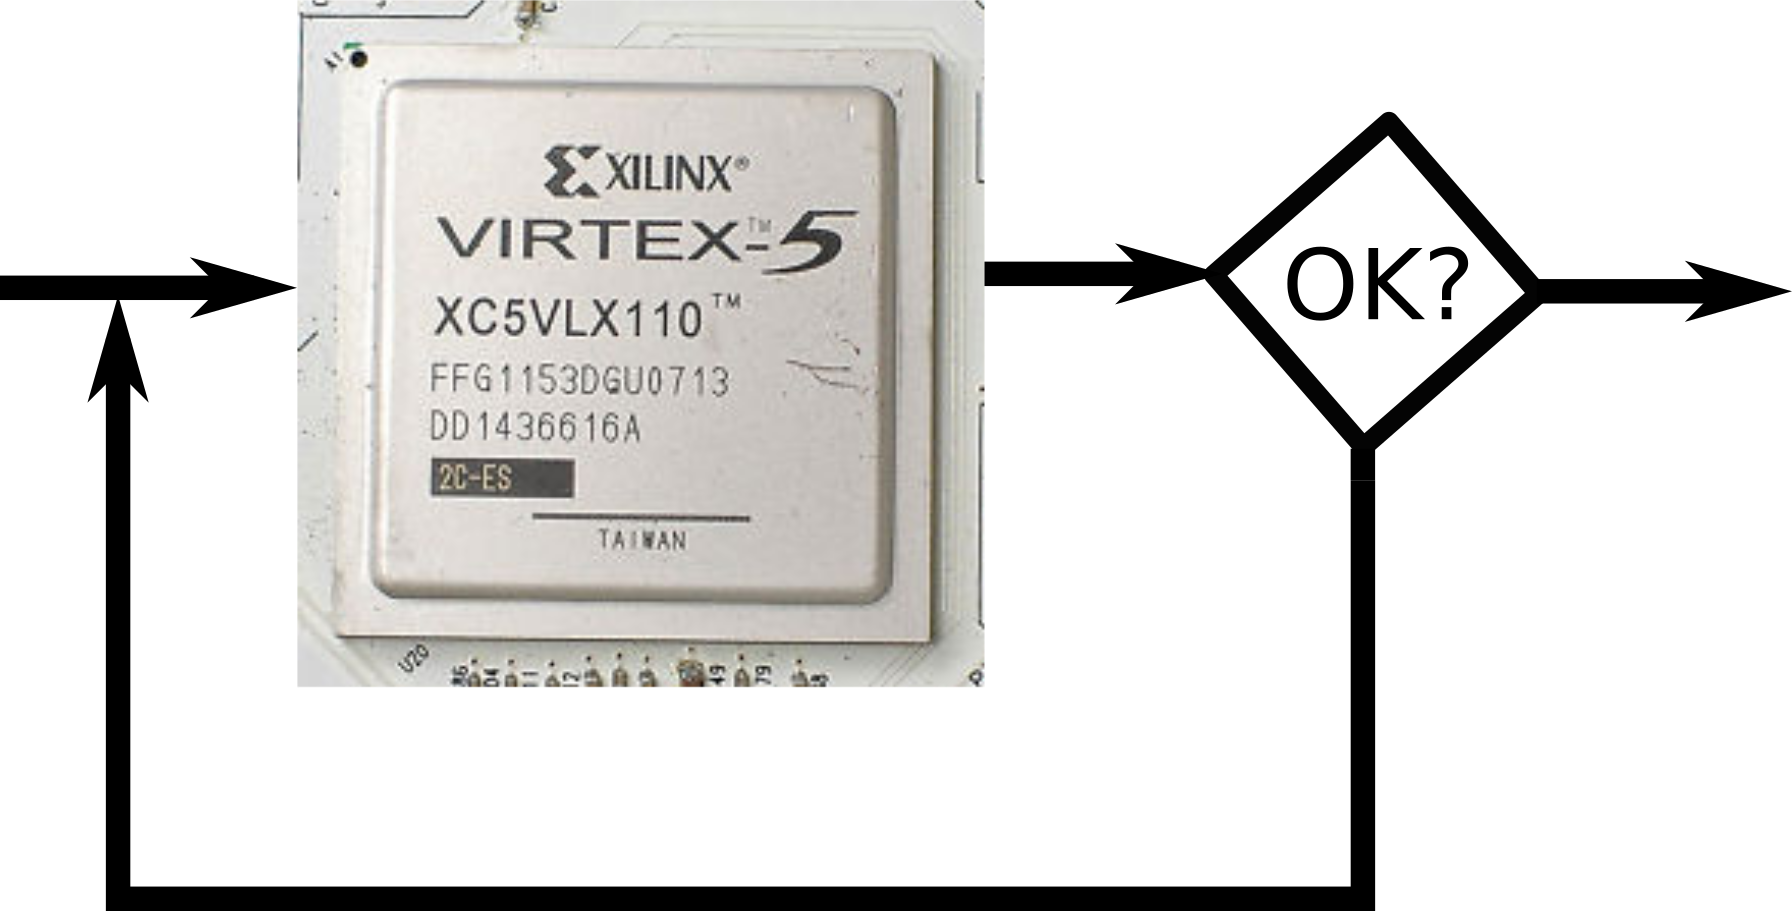
\includegraphics[scale=0.26]{./figures/fpga_design.png}
% 	  \end{center}
%   }
% 
% \end{frame}
% 
% \begin{frame}
% 	\begin{center}
% 	\Huge MOTIVACIÓN Y OBJETIVOS
% 	\end{center}
% \end{frame}
% 
% \subsection{Motivacion}
% 
% \begin{frame}{Motivación}
%   \Fontit
%   \begin{itemize}
%     \item<1-> El avance de los sistemas de radio definidos por software
%     \item<2-> La flexibilidad que brindan las FPGAs para implementar sistemas complejos
%     \item<3-> La necesidad de sistemas de comunicaciones de código libre, eficientes y económicos
%     \item<4-> Aportar al desarrollo de un sistema de telecomunicaciones dentro del LSE
%     de la facultad
%   \end{itemize}
% \end{frame}
% 
\subsection{Objetivos}
\begin{frame}{Objetivos}
  \Fontit
  \begin{itemize}
    \item<1-> Dise�ar un modulador/demodulador OFDM para un sistema de telecomunicaciones definido por
    software que cumpla con el estandard ISDB-T.
    \item<2-> Que sirva tambi�n como unidad de c�mputo FFT/IFFT para procesamiento de se�ales. 
    \item<3-> Requerimientos
    \only<4-9>{
      \begin{itemize}
          \Fontitit
		  \item<4-9> Longitud configurable, incluyendo al menos 2K, 4K y 8K muestras (ISDB-T).
		  \item<5-9> Frecuencia de muestreo m�nima de $8,126,984$ muestras garantizada (ISDB-T).
		  \item<6-9> Entrada y salida continua.
		  \item<7-9> Aritm�tica de punto fijo.
		  \item<8-9> Unidad de escalamiento configurable en ejecuci�n con opci�n de seleccionar la etapa a escalar y el m�todo (redondeo/truncamiento).
		  \item<9-9> Menor consumo de espacio/recursos que otras implementaciones (ref: Xilinx IP FFT 7.0 y un core FFT abierto dise�ado para modulaci�n OFDM ISDB-T).
	  \end{itemize}}
    \item<10-> Realizar una evaluaci�n de desempe�o
    \only<11-14>{\begin{itemize}
      \Fontitit
      \item<11-14> Funcionamiento
      \item<12-14> Ruido / error
      \item<13-14> Distorsi�n arm�nica
      \item<14-14> Recursos
    \end{itemize}}
    \item<15-> Realizar una comparativa con desarrollos de terceros para evaluar el dise�o realizado
    \item<16-> Proponer trabajos futuros para continuar y mejorar el dise�o.
 \end{itemize}
\end{frame}

\section{Selecci�n de las arquitecturas}

\begin{frame}
    \begin{center}
	\Huge SELECCI�N DE LAS ARQUITECTURAS
	\end{center}
\end{frame}

\subsection{Transformada de Fourier}

\begin{frame}{Arquitectura}
	\begin{itemize}
	    \Fontit
	    \item<1-> Algoritmo: Radix-r
	    \begin{itemize}
	      \Fontitit
	      \item<2-> Flexibilidad en la longitud
	      \item<3-> Simplicidad en la implementaci�n
	      \item<4-> Posibilidad de reutilizar m�dulos
	    \end{itemize} 
	    \item<5-> Longitud del bloque: 2 y 4
	    \begin{itemize}
	      \Fontitit
	      \item<6-> No implican multiplicaciones no triviales (solo por twiddle factors)
	    \end{itemize}
	    \item<7-> Implementaci�n: arquitectura iterativa
	    \begin{itemize}
	      \item<8-> Un solo bloque para todos los c�lculos
	      \item<9-> Es la implementaci�n m�s peque�a (requerimiento)
	      \item<10-> Se computa una etapa a la vez
	    \end{itemize}
	\end{itemize}
	\uncover<11->{
      \begin{center}
	    \advance\leftskip-0.2cm
	    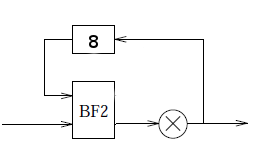
\includegraphics[scale=0.375]{./figures/r2sBf.png}
      \end{center}
     }
	
\end{frame}
  %\begin{block}{Comparativa de los algoritmos FFT}
%   \begin{itemize}
%     \item<1-> Comparativa de los algoritmos FFT
% 	\begin{center}
% 	  \advance\leftskip-0.2cm
% 	  {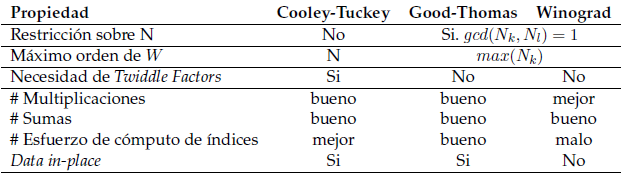
\includegraphics[scale=0.45]{./figures/FFT_table.png}}
%     \end{center}
%   %\end{block}
%   
%   \item<2-> Selección
%     \begin{itemize}
%       \item<2-> Se decide implementar una arquitectura basada en el algoritmo
%       Cooley-Tuckey.
%       \item<3-> Se implementará la versión del algoritmo en que los sub-cómputos son del mismo
%       tamaño, conocidos como radix-r.
%     \end{itemize}
%   \end{itemize}
%   \begin{itemize}
%     \Fontit
%     \item<1-> Existen varios algoritmos
%     \begin{itemize}
%       \Fontitit
%       \item<2-> Good-Thomas
%       \item<3-> Winograd
%       \item<4-> Cooley-Tuckey
%     \end{itemize} 
%     \item<5-> Se selecciona el algoritmo Radix-r (Cooley-Tuckey)
%     \begin{itemize}
%       \Fontitit
%       \item<6-> Flexibilidad en la longitud
%       \item<7-> Simplicidad en la implementaci�n
%       \item<8-> Posibilidad de reutilizar m�dulos
%     \end{itemize}
%   \end{itemize}
% \end{frame}
% 
% \begin{frame}{Cantidad de puntos por operaci�n}
%   \begin{itemize}
% %     \item<1-> A mayor longitud de las DFTs interiores es menor la cantidad de DFTs interiores a
% %     realizar. Pero aumentan la cantidad de operaciones por DFT.
%     \item<1-> Cantidad de etapas
%     \item<2-> Cantidad de operaciones por etapa
%     \vfill
%     
%     \uncover<3->{\begin{tabular}{c c c c}
% 		\textbf{Long. del bloque} & \textbf{Mult.} & \textbf{Mult. no triv} &
% 		\textbf{sumas} \\ \hline 
% 		$2$ & $2$ & \color<3->[rgb]{1,0,0}$0$ & $2$ \\
% 		$3$ & $3$ & $2$ & $6$ \\
% 		$4$ & $4$ & \color<3->[rgb]{1,0,0}$0$ & $8$ \\
% 		$5$ & $6$ & $5$ & $17$ \\
% 		$7$ & $9$ & $8$ & $36$ \\
% 		$8$ & $8$ & $2$ & $26$ \\
% 		$9$ & $11$ & $10$ & $44$ \\ \hline
%     \end{tabular}}
%     
%     \vfill
% 
%   \item<4-> Se decide implementar dos arquitecturas: radix-2 y radix-4
%   \end{itemize}
% \end{frame}
% 
% % \begin{frame}{Arquitecturas para la implementación radix-r}
% %   \begin{block}{Esquema radix-2 de 8 puntos}<1->
% %      \begin{center}
% % 	  \advance\leftskip-0.2cm
% % 	  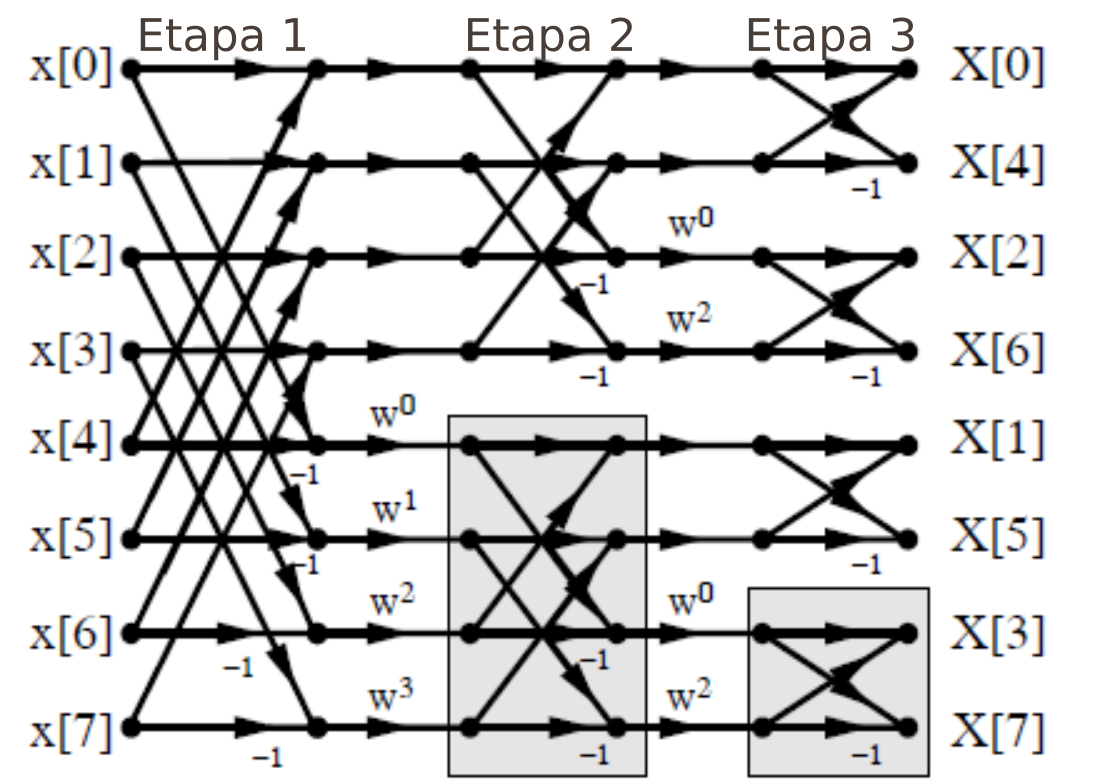
\includegraphics[scale=0.42]{./figures/r2_8.png}
% %     \end{center}
% %   \end{block}
% %   
% %   %\only<2-3>{
% %   \begin{itemize}
% %     \item<2-> Cada círculo representa una suma
% %     \item<3-> Cada flecha representa un producto
% %   \end{itemize}
%   %}
% %\end{frame}}
%   
% %   \only<4-5>{
% %   \begin{itemize}
% %     \item<4-> Existen varias alternativas de implementación de este algoritmo
% %     \item<5-> Se diferencian en la forma en que se procesan las etapas del esquema
% %   \end{itemize}}
% %\end{frame}
% 
% \begin{frame}{Arquitecturas para la implementaci�n radix-r}
%   \begin{itemize}
%     \item<1-> Arquitectura paralela
%     \uncover<2-5>{
%       \begin{center}
% 	    \advance\leftskip-0.2cm
% 	    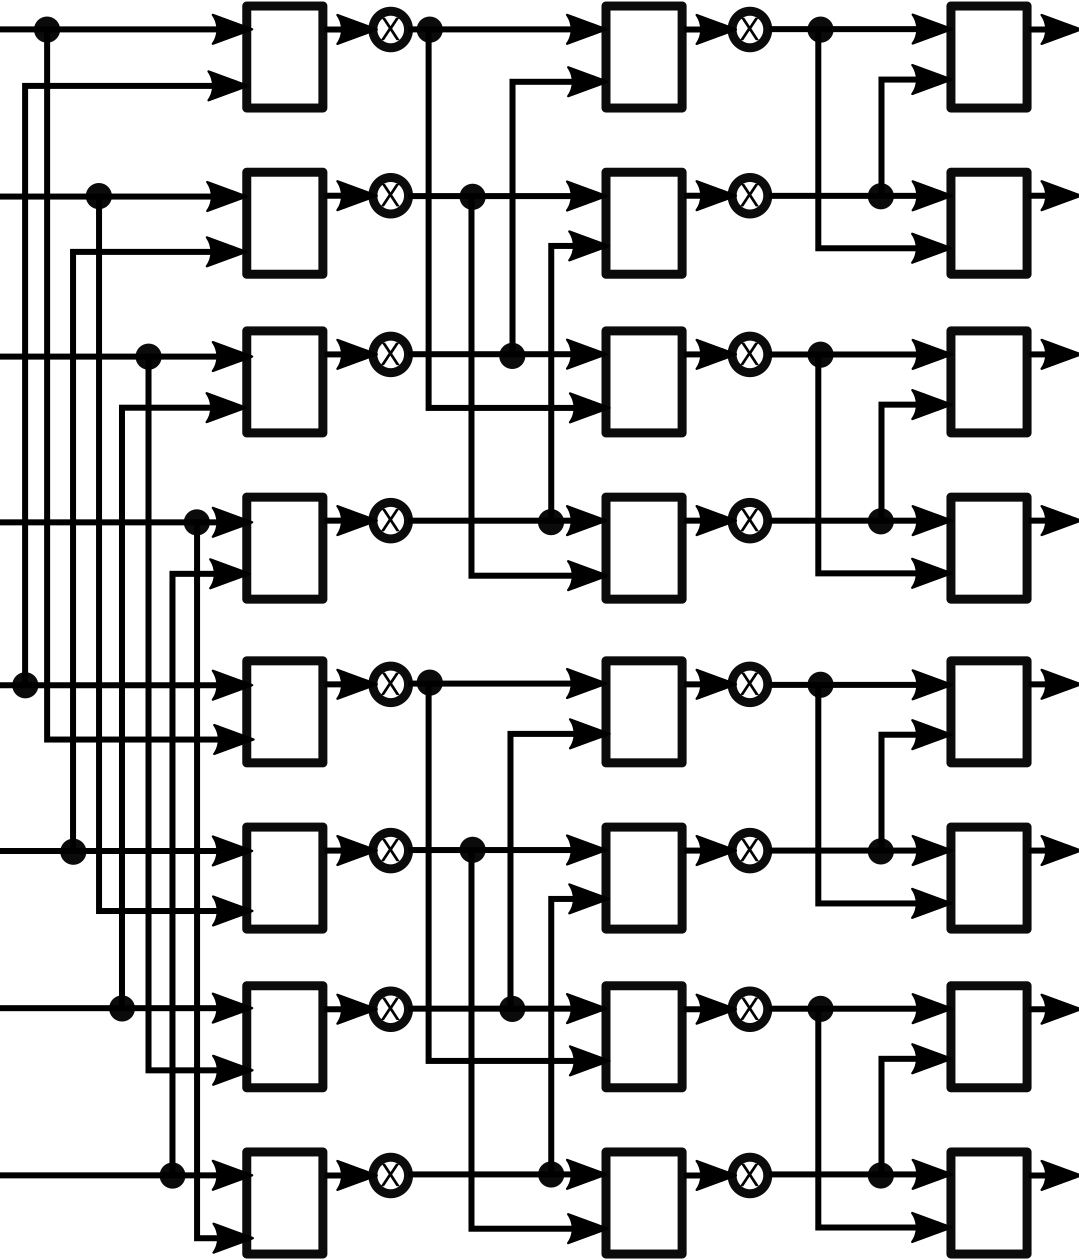
\includegraphics[scale=0.155]{./figures/r2_paralel.png}
%       \end{center}
%     }
%     \item<1-> Arquitectura desenrrollada
%     \uncover<3-5>{
%       \begin{center}
% 	    \advance\leftskip-0.2cm
% 	    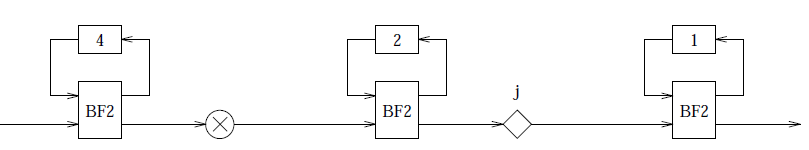
\includegraphics[scale=0.275]{./figures/r2sdf_8.png}
%       \end{center}
% %     \begin{itemize}
% %       \item<8-> Un butterfly y un multiplicador por cada etapa
% %       \item<9-> Bus serie
% %       \item<10-> Pipeline
% %     \end{itemize}
%      }
%     \item<1-> Arquitectura iterativa
%     \uncover<4-5>{
%       \alt<4>{
%       \begin{center}
% 	    \advance\leftskip-0.2cm
% 	    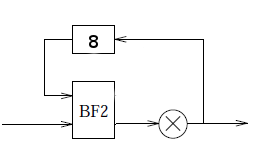
\includegraphics[scale=0.375]{./figures/r2sBf.png}
%       \end{center}
%       }{
%       \begin{center}
% 	    \advance\leftskip-0.2cm
% 	    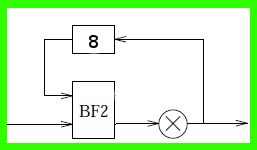
\includegraphics[scale=0.375]{./figures/r2sBf_sel2.png}
%       \end{center}
%       }
% %     \begin{itemize}
% %       \item<13-> Un único buterfly y un único multiplicador para todas las etapas
% %     \end{itemize}
%      }
%   \end{itemize}
% \end{frame}

% \begin{frame}{Selección de arquitectura radix}
%   \begin{center}
%     \advance\leftskip-0.2cm
%     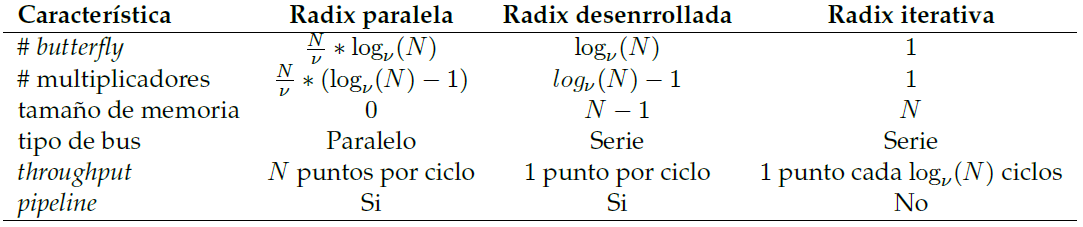
\includegraphics[scale=0.27]{./figures/radix_table.png}
%   \end{center}
%   
%   \begin{itemize}
%     \item<2-> Dado el requerimiento de la economía espacial y de recursos
% %     \item<3-> Y dado que el trhoughput no es fundamental
%     \item<3-> Se selecciona la arquitectura iterativa para la implementación de las arquitecturas
%     radix-2 y radix-4.
%   \end{itemize}
% \end{frame}

\section{Implementaci�n}

\begin{frame}
\begin{center}
\Huge IMPLEMENTACI�N DE LAS ARQUITECTURAS
\end{center}
\end{frame}

\subsection{Arquitecturas radix}

\begin{frame}{Radix-2 Iterativa}
  \begin{columns}[T]
    \uncover<1->{
    \begin{column}{.5\textwidth}
      \begin{center}
	    \advance\leftskip-0.2cm
	    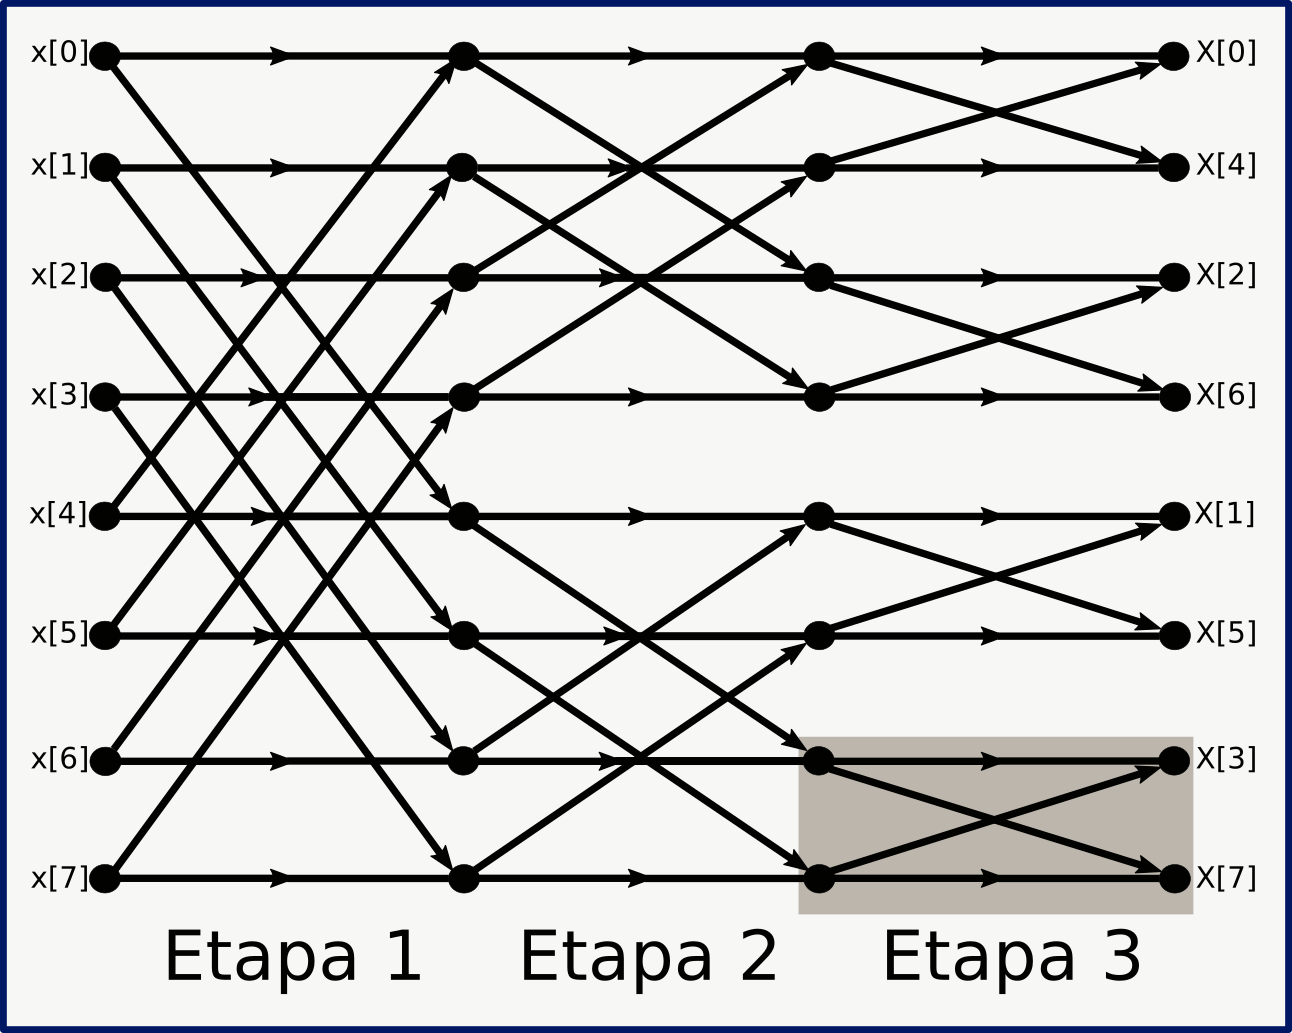
\includegraphics[scale=0.28]{./figures/r2_8_diag.png}
      \end{center}
    \end{column}
    }
    
    \uncover<2->{
    \begin{column}{.5\textwidth}
      \begin{center}
	    \advance\leftskip-0.2cm
	    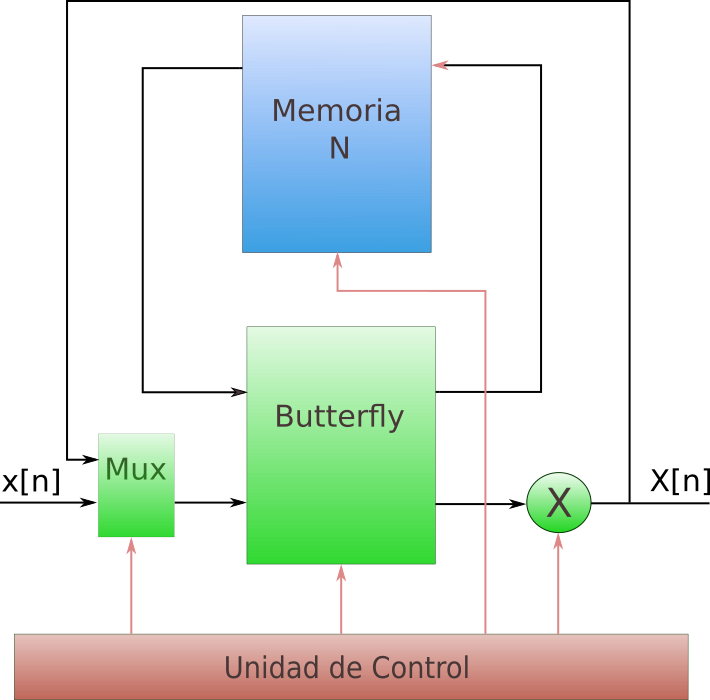
\includegraphics[scale=0.23]{./figures/radix2blocks.png}
      \end{center}
    \end{column}
    }
  \end{columns}
  
%   \begin{itemize}
%     \item<3-> Memoria
%     \item<4-> Butterfly (sumador/restador + escalamiento)
%     \item<5-> Producto por los \textit{twiddle factors}
%     \item<6-> Datapath 
%     \item<7-> Unidad de control
%   \end{itemize}  
    
\end{frame}

\begin{frame}{Radix-4 Iterativa}

%   \only<1-1>{
%    \vfill
%     \begin{center}
%       \advance\leftskip-0.2cm
%       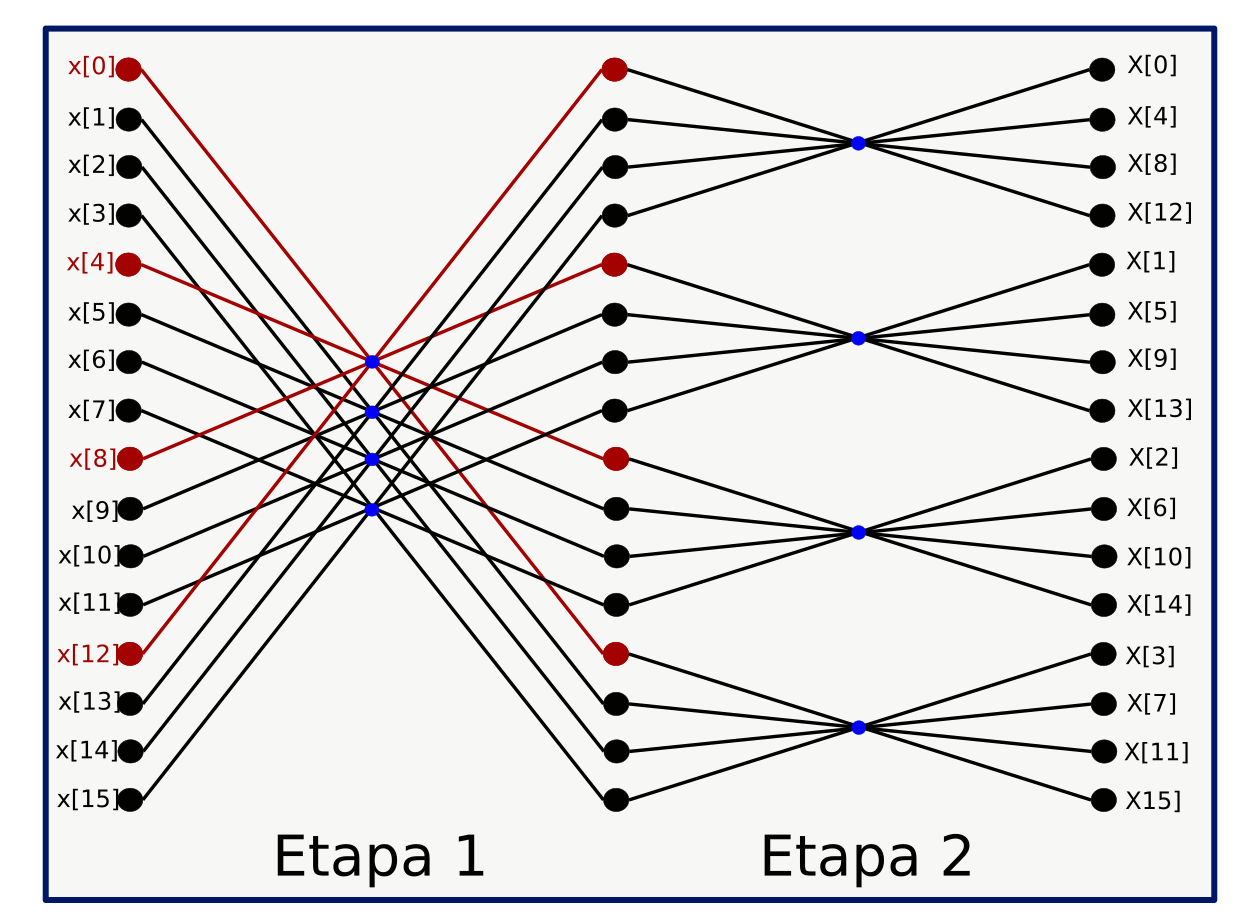
\includegraphics[scale=0.43]{./figures/r4_16.png}
%     \end{center}
%     \vfill
%   }
  
  \begin{columns}[T]
    \uncover<1->{
    \begin{column}{.5\textwidth}
      \begin{center}
	    \advance\leftskip-0.2cm
	    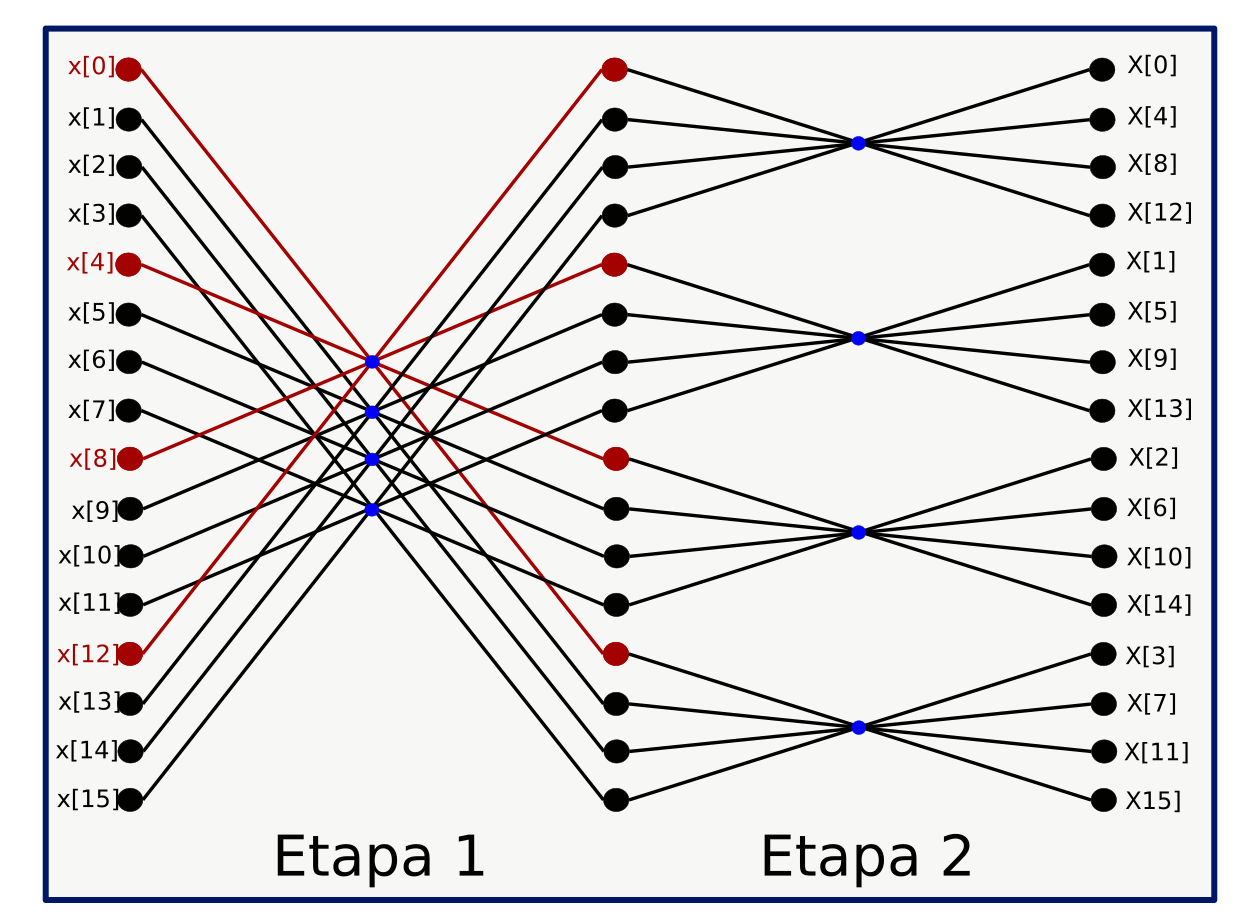
\includegraphics[scale=0.3]{./figures/r4_16.png}
      \end{center}
    \end{column}
    }
    
    \uncover<2->{
    \begin{column}{.5\textwidth}
      \begin{center}
	    \advance\leftskip-0.2cm
	    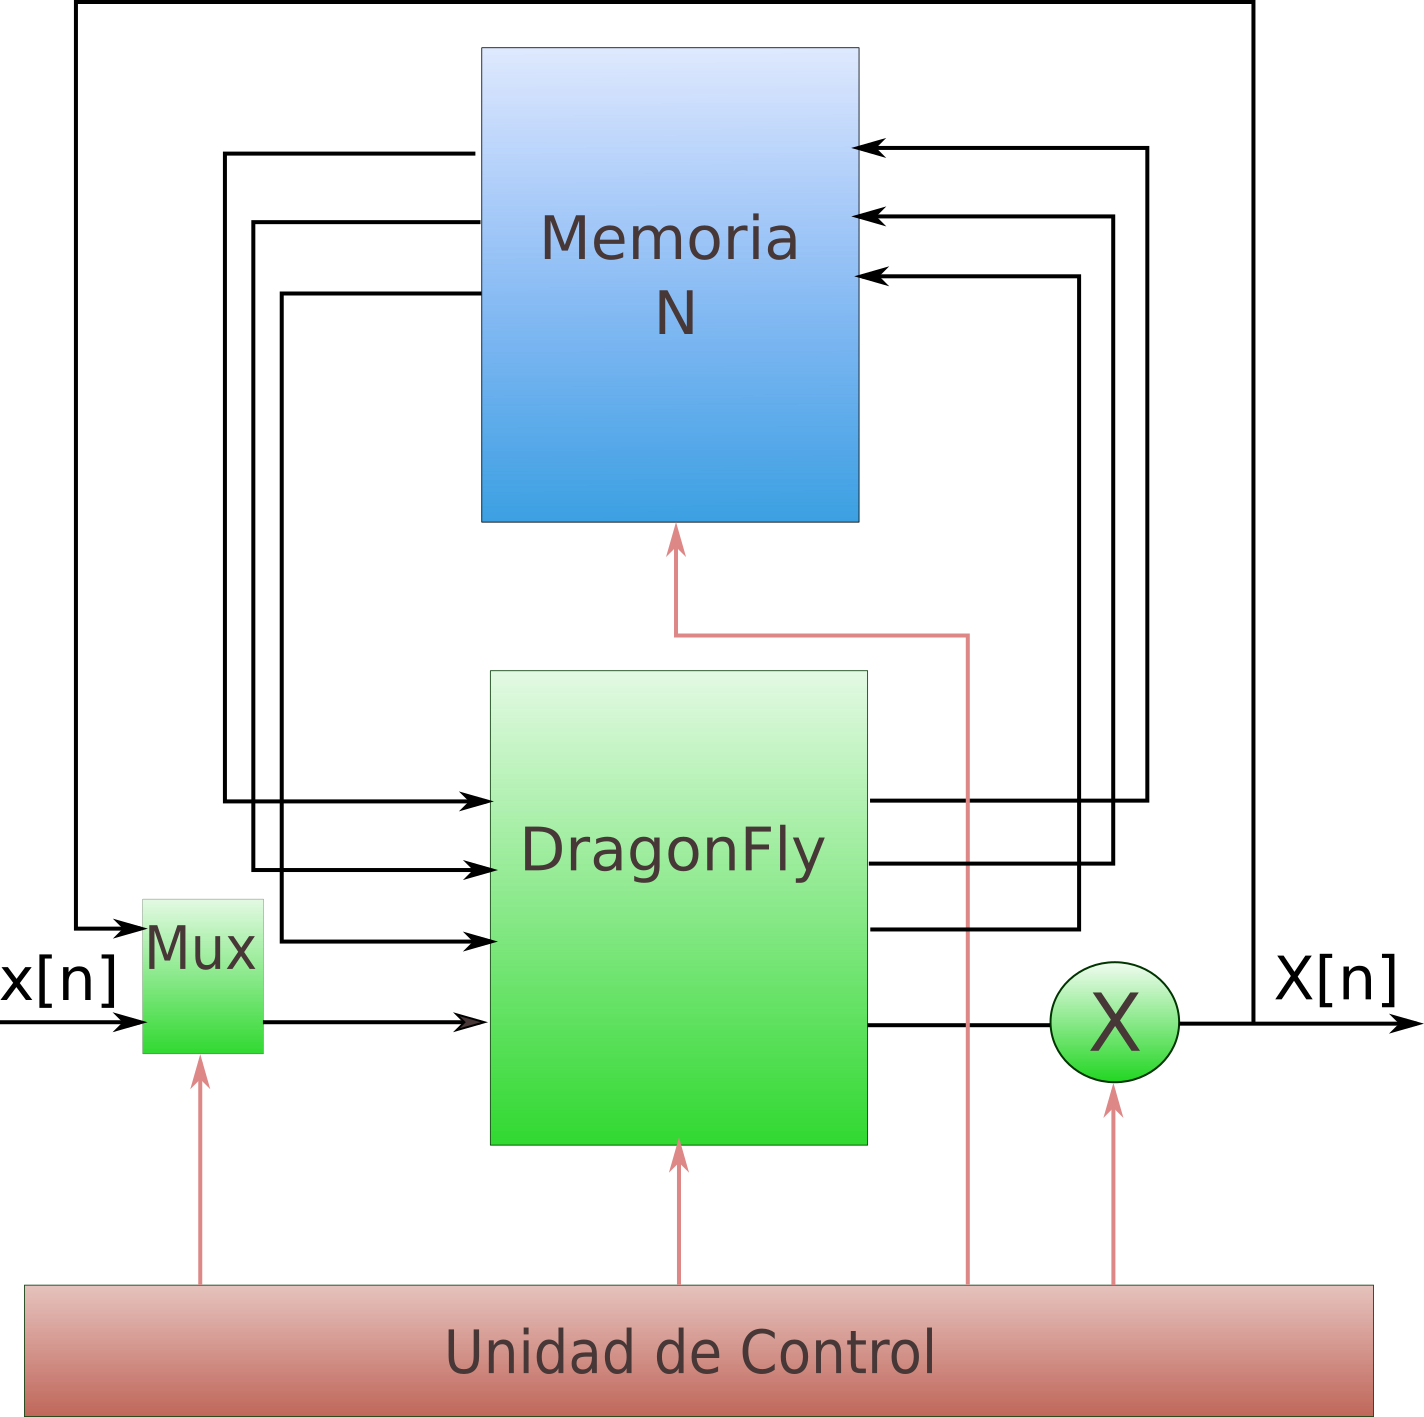
\includegraphics[scale=0.23]{./figures/radix4blocks.png}
      \end{center}
    \end{column}
    }
  \end{columns}
  
%   \begin{itemize}
%     \item<3-> Memoria
%     \item<4-> Butterfly (sumador/restador + escalamiento)
%     \item<5-> Producto por los \textit{twiddle factors}
%     \item<6-> Datapath 
%     \item<7-> Unidad de control
%   \end{itemize}  
    
\end{frame}
  
\begin{frame}
   
   \begin{columns}[T]
    \uncover<1->{
    \begin{column}{.5\textwidth}
      \begin{center}
	    \advance\leftskip-0.2cm
	    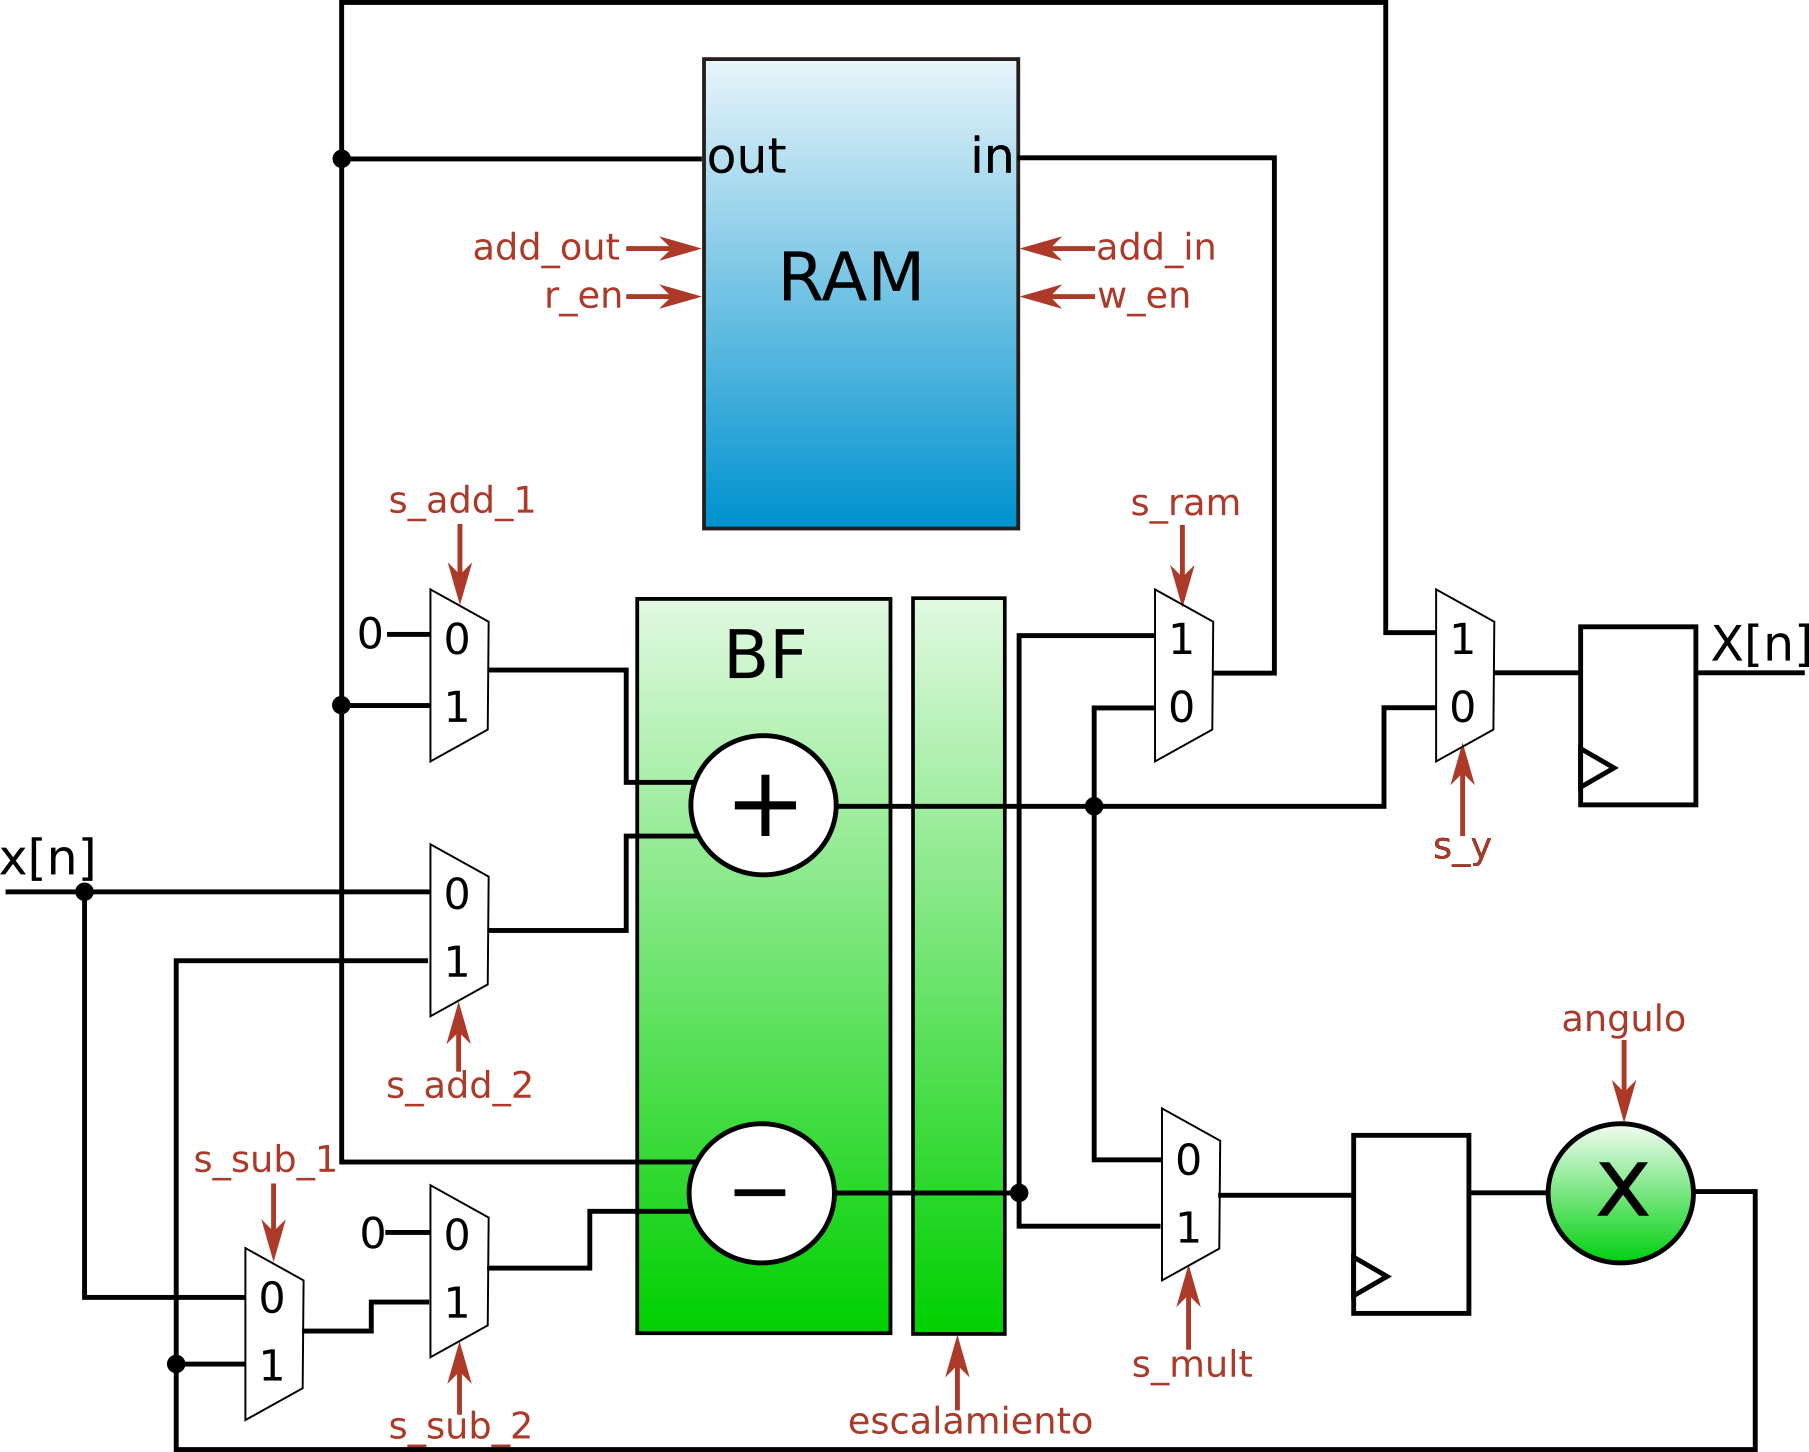
\includegraphics[scale=0.275]{./figures/datapathMem.png}
      \end{center}
    \end{column}
    }
    
    \uncover<1->{
    \begin{column}{.5\textwidth}
      \begin{center}
	    \advance\leftskip-0.2cm
	    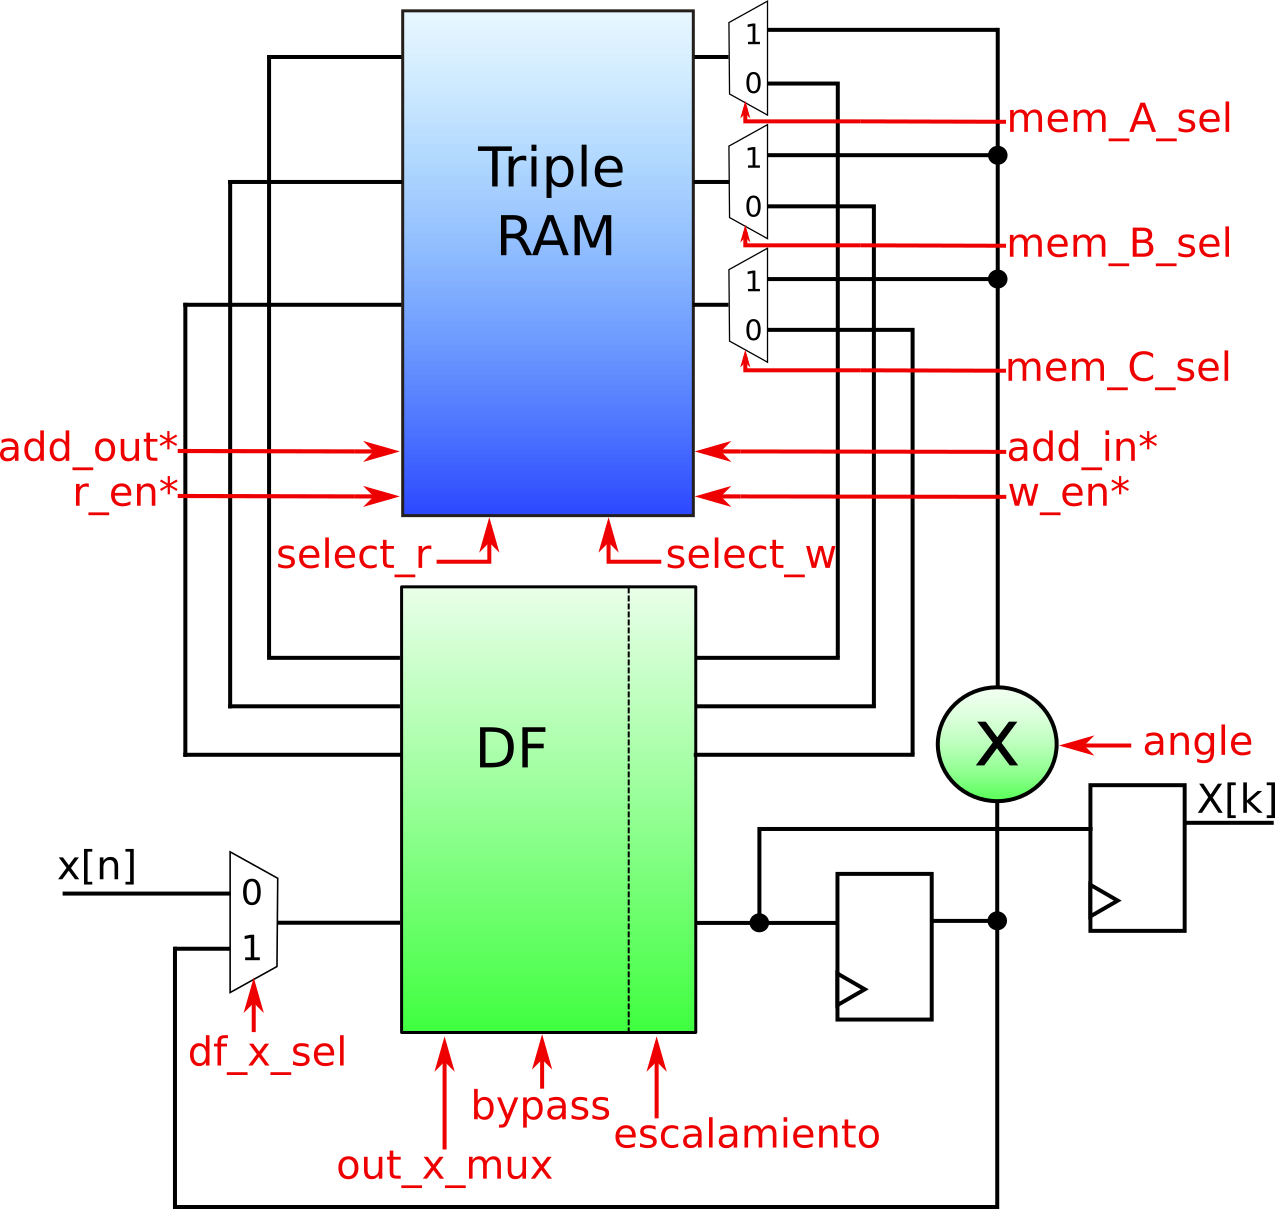
\includegraphics[scale=0.272]{./figures/r4control.png}
      \end{center}
    \end{column}
    }
  \end{columns}
  
  \begin{columns}[T]
  \begin{column}{.2\textwidth}
  \end{column}
  \begin{column}{.6\textwidth}
  \begin{center} 
    \begin{itemize}
      \item<2-> Unidad aritm�tica (incluyendo unidad de escalamiento)
      \item<3-> Multiplicador
	  \only<4-5>{
	      \begin{itemize}
	        \item<4-> Algoritmo Cordic
	        \item<5-> Multiplicador comlejo eficiente
	      \end{itemize}
	  } 
      \item<6-> Memoria
      \only<7-8>{
	      \begin{itemize}
	        \item<7-> Radix-2: Dual-port RAM
	        \item<8-> Radix-4: Triple in/Triple out RAM
	      \end{itemize}
	  }
      \item<9-> Datapath
      \item<10-> Unidad de control
    \end{itemize}
  \end{center}
  \end{column}
  \begin{column}{.2\textwidth}
  \end{column}
  \end{columns}
\end{frame}

% \subsection{Unidad aritmética}
% \begin{frame}{}
%   \begin{columns}[T]
%     \uncover<1->{
%     \begin{column}{.5\textwidth}
%       \begin{itemize}
%         \item<1-> Suma y resta entre dos puntos         
%       \end{itemize}
%       \uncover<2->{
%         \begin{center}
%         \advance\leftskip-0.2cm
%         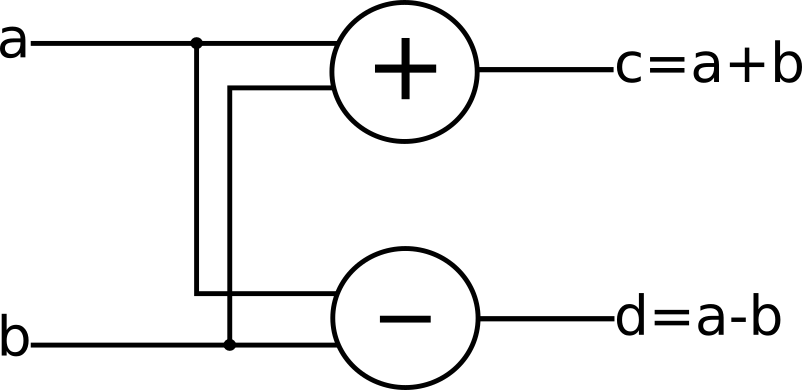
\includegraphics[scale=0.45]{./figures/butterfly_esq.png}
%       \end{center}
%       }
%     \end{column}
%     }
%     
%     \uncover<3->{
%     \begin{column}{.5\textwidth}
%       \begin{itemize}
%         \item<3-> Operaciones entre cuatro puntos
%         \item<4-> Datapath interno          
%       \end{itemize}
%       \uncover<5->{
%         \begin{center}
%         \advance\leftskip-0.2cm
%         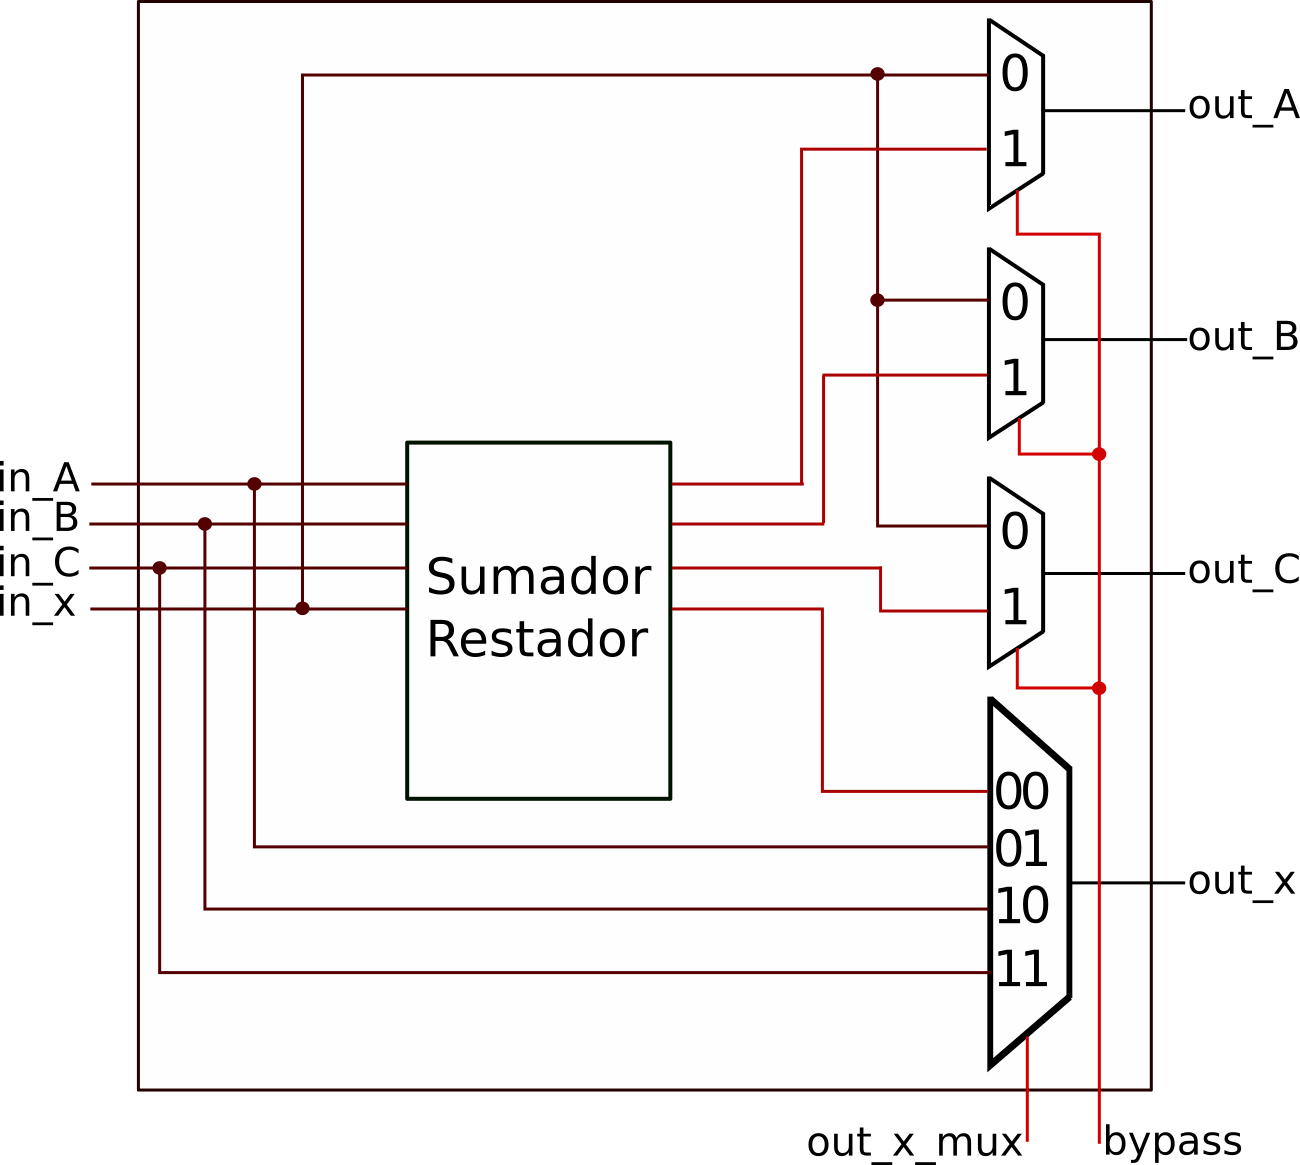
\includegraphics[scale=0.25]{./figures/firefly.png}
%       \end{center}
%       }
%     \end{column}
%     }
%     \end{columns}
%   
% \end{frame}
% 
% \subsection{Multiplicación}
% 
% \begin{frame}{Algoritmo Cordic}
%   \begin{itemize}
%     \item<1-> Rotaciones en base a microrotaciones
%     \item<2-> Microrotaciones sucesivas
%     \item<4-> Arquitectura desenrrollada
% %     \begin{itemize}
% %       \item<2-> Permite realizar todo el procesamiento en un solo ciclo de clock
% %       \item<3-> Permite la implementación de un \textit{pipeline} entre las etapas de rotación
% %     \end{itemize}
%     \item<5-> Preprocesador
%     \item<6-> Escalado final
%   \end{itemize}
%   
%   \begin{columns}[T]
%     \uncover<3-8>{
%       \begin{column}{.3\textwidth}
%          \begin{center}
%            \advance\leftskip-0.2cm
%            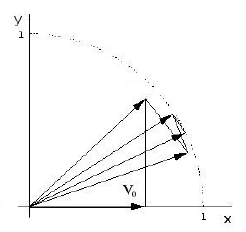
\includegraphics[scale=0.45]{./figures/cordic.png}
%          \end{center}
%       \end{column}
%     }
%     \begin{column}{.6\textwidth} 
%       \only<7-7>{
%         \begin{center}
%           \advance\leftskip-0.2cm
%           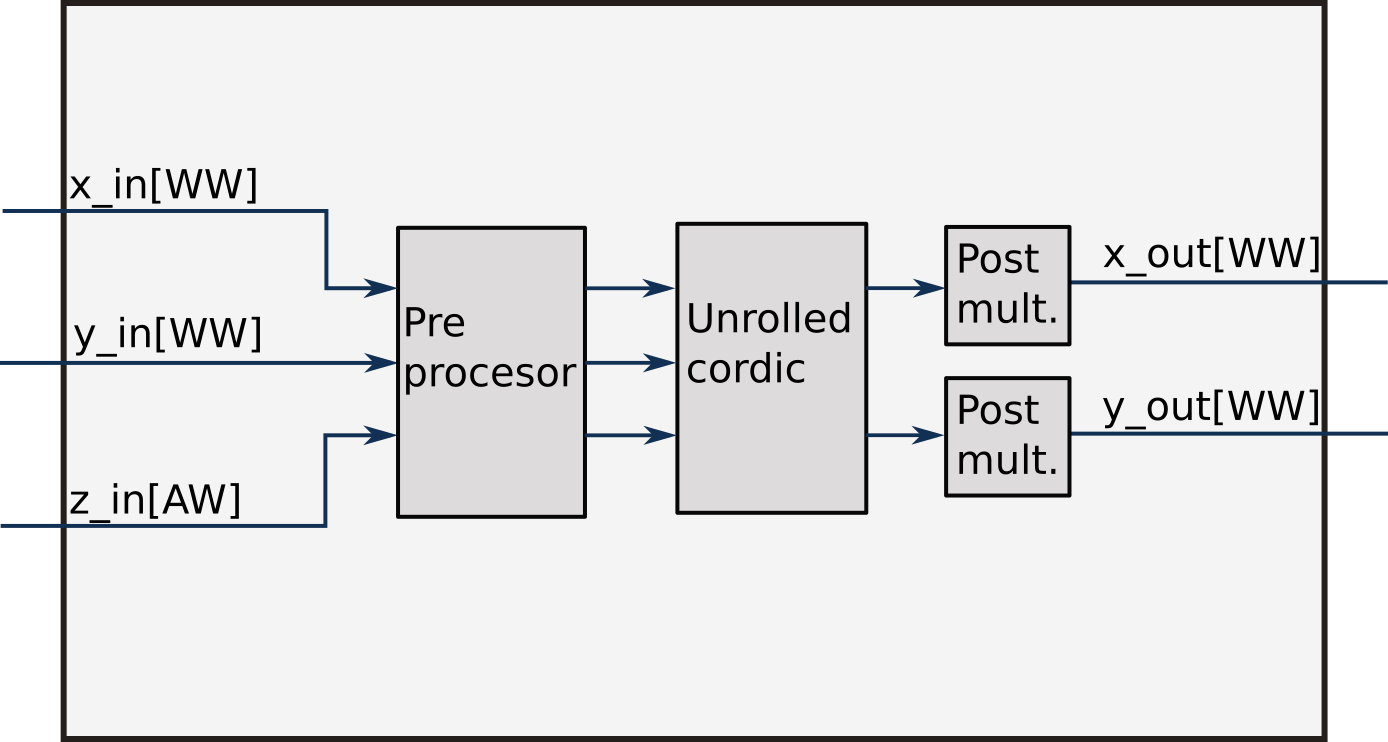
\includegraphics[scale=0.3]{./figures/cordicBlocks.png}
%         \end{center}
%       }
%       \only<8-8>{
%         \begin{center}
%           \advance\leftskip-0.2cm
%           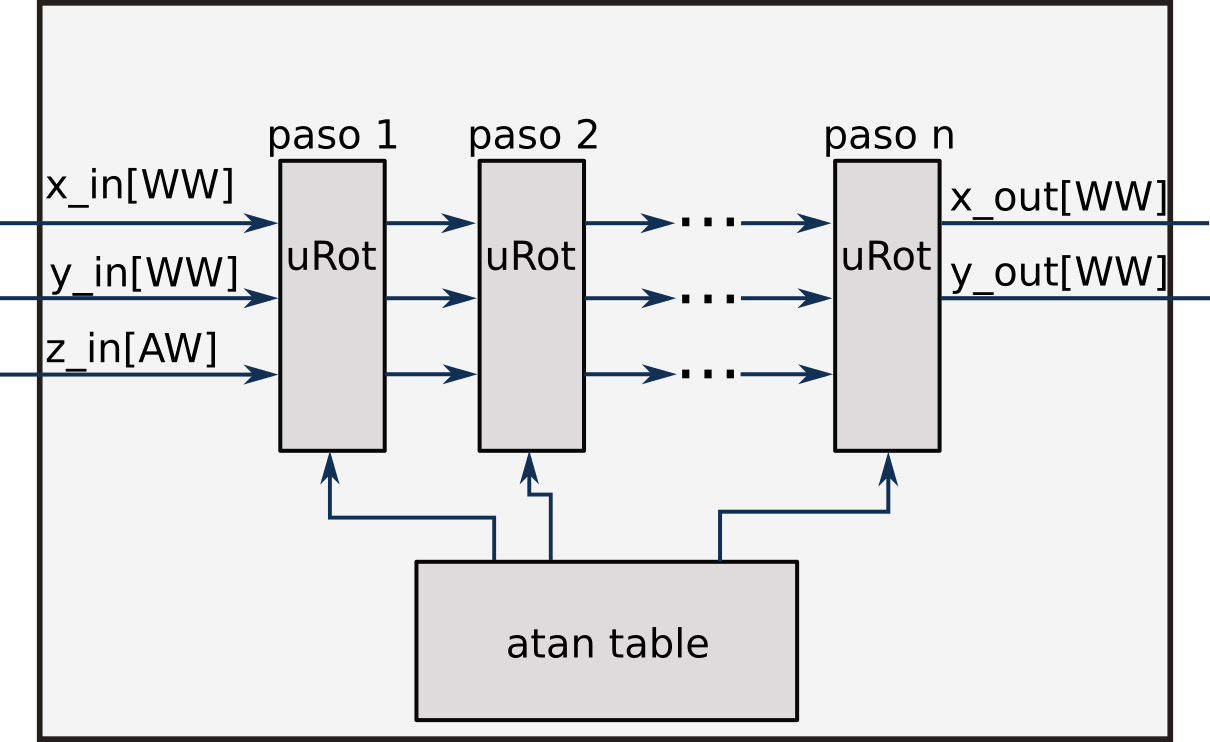
\includegraphics[scale=0.3]{./figures/uCordicBlocks.png}
%         \end{center}
%       }
%     \end{column}
%   \end{columns}
% \end{frame}
% 
% \begin{frame}{Multiplicador complejo}
% \begin{itemize}
%   \item<1-> Memoria para los factores
%   \item<2-> Preprocesador
%   \item<3-> Multiplicación compleja
%   \uncover<4->{
%   \begin{center}
%     \advance\leftskip-0.2cm
%     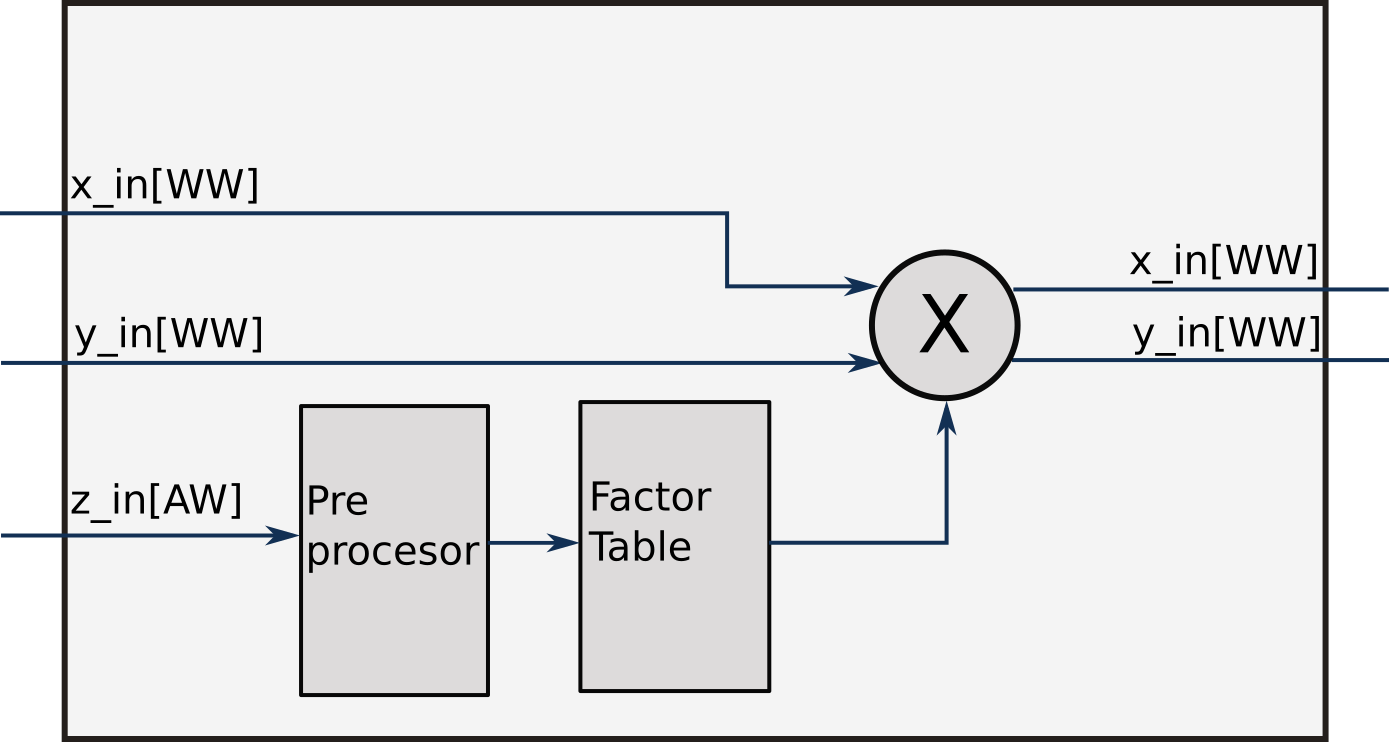
\includegraphics[scale=0.3]{./figures/multBlocks.png}
%   \end{center}
%   }
% \end{itemize}
% \end{frame}
% 
% \subsection{Memoria}
% \begin{frame}{}
% 
%   \begin{columns}[T]
%     \uncover<1->{
%     \begin{column}{.5\textwidth}
%       \begin{center}
% 	    \advance\leftskip-0.2cm
% 	    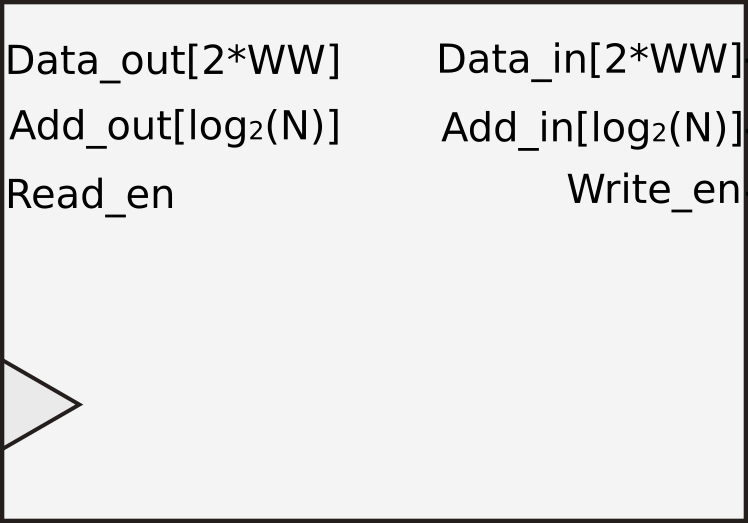
\includegraphics[scale=0.3]{./figures/dportRam.png}
%       \end{center}
%       
%       \begin{itemize}
%         \item<2-> Tipo dual port RAM
%         \item<3-> Un puerto de lectura y uno de esccritura
%       \end{itemize}
%     \end{column}
%     }
%     
%     \uncover<1->{
%     \begin{column}{.5\textwidth}
%       \begin{center}
% 	    \advance\leftskip-0.2cm
% 	    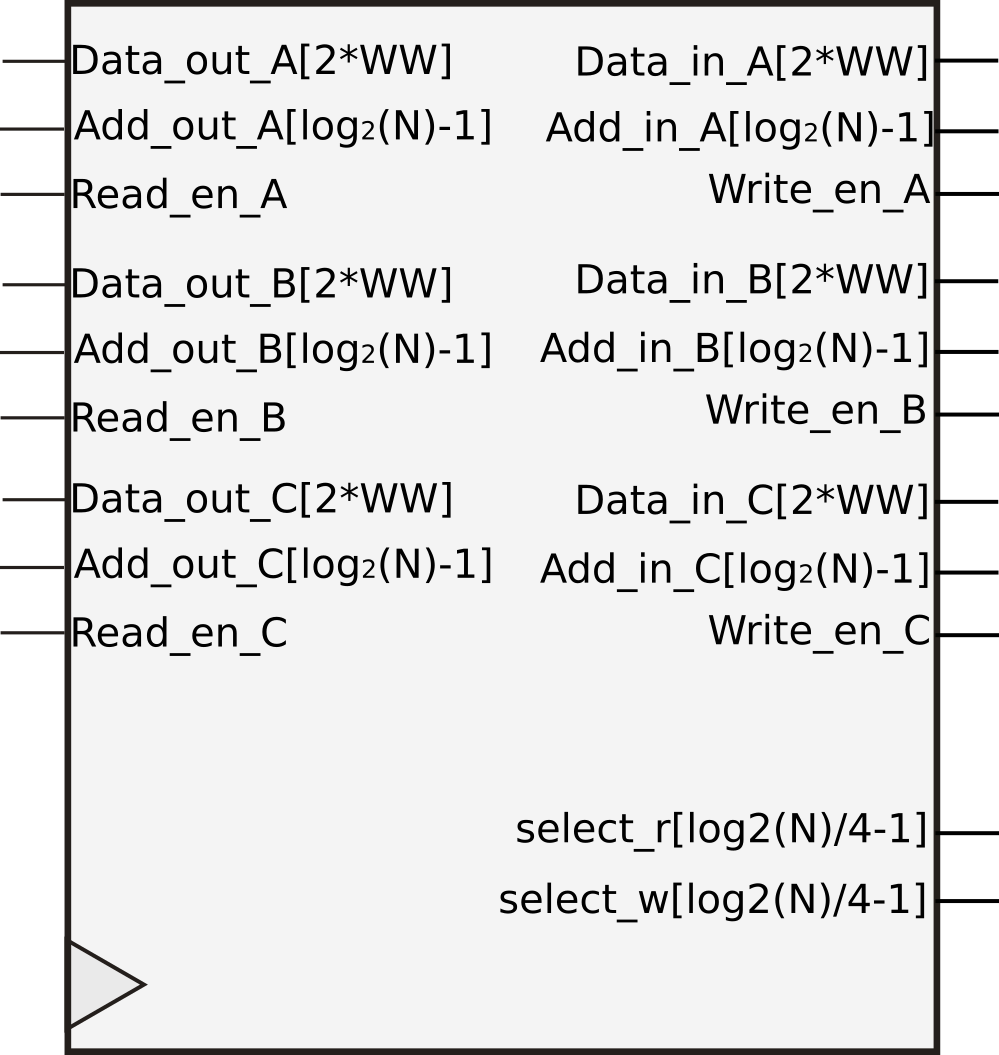
\includegraphics[scale=0.23]{./figures/tripleRAM.png}
%       \end{center}
%       \begin{itemize}
%         \item<4-> En cada operación se necesitan leer tres datos y escribir tres datos
%         \item<5-> Tres puertos de lectura y tres puertos de escritura
%         \item<6-> tres sub-bloques dual port RAM
%       \end{itemize}
%       \end{column}
%      }
%     
%     \end{columns}
%   
% \end{frame}
% 
% \subsection{Datapath}
% \begin{frame}{Datapath general}
% 
%   \begin{itemize}
%     \item<1-> Hay dos tipos de operaciones posibles
%     \begin{itemize}
%       \Fontitit
%       \item<2-> Traspaso de datos en memoria
%       \item<3-> Operación aritmética entre dos datos
%     \end{itemize}
%   \end{itemize}
%   
%   \begin{columns}[T]
%     \uncover<4->{
%       \begin{column}{.5\textwidth}
%         \begin{center}
%           \advance\leftskip-0.2cm
%           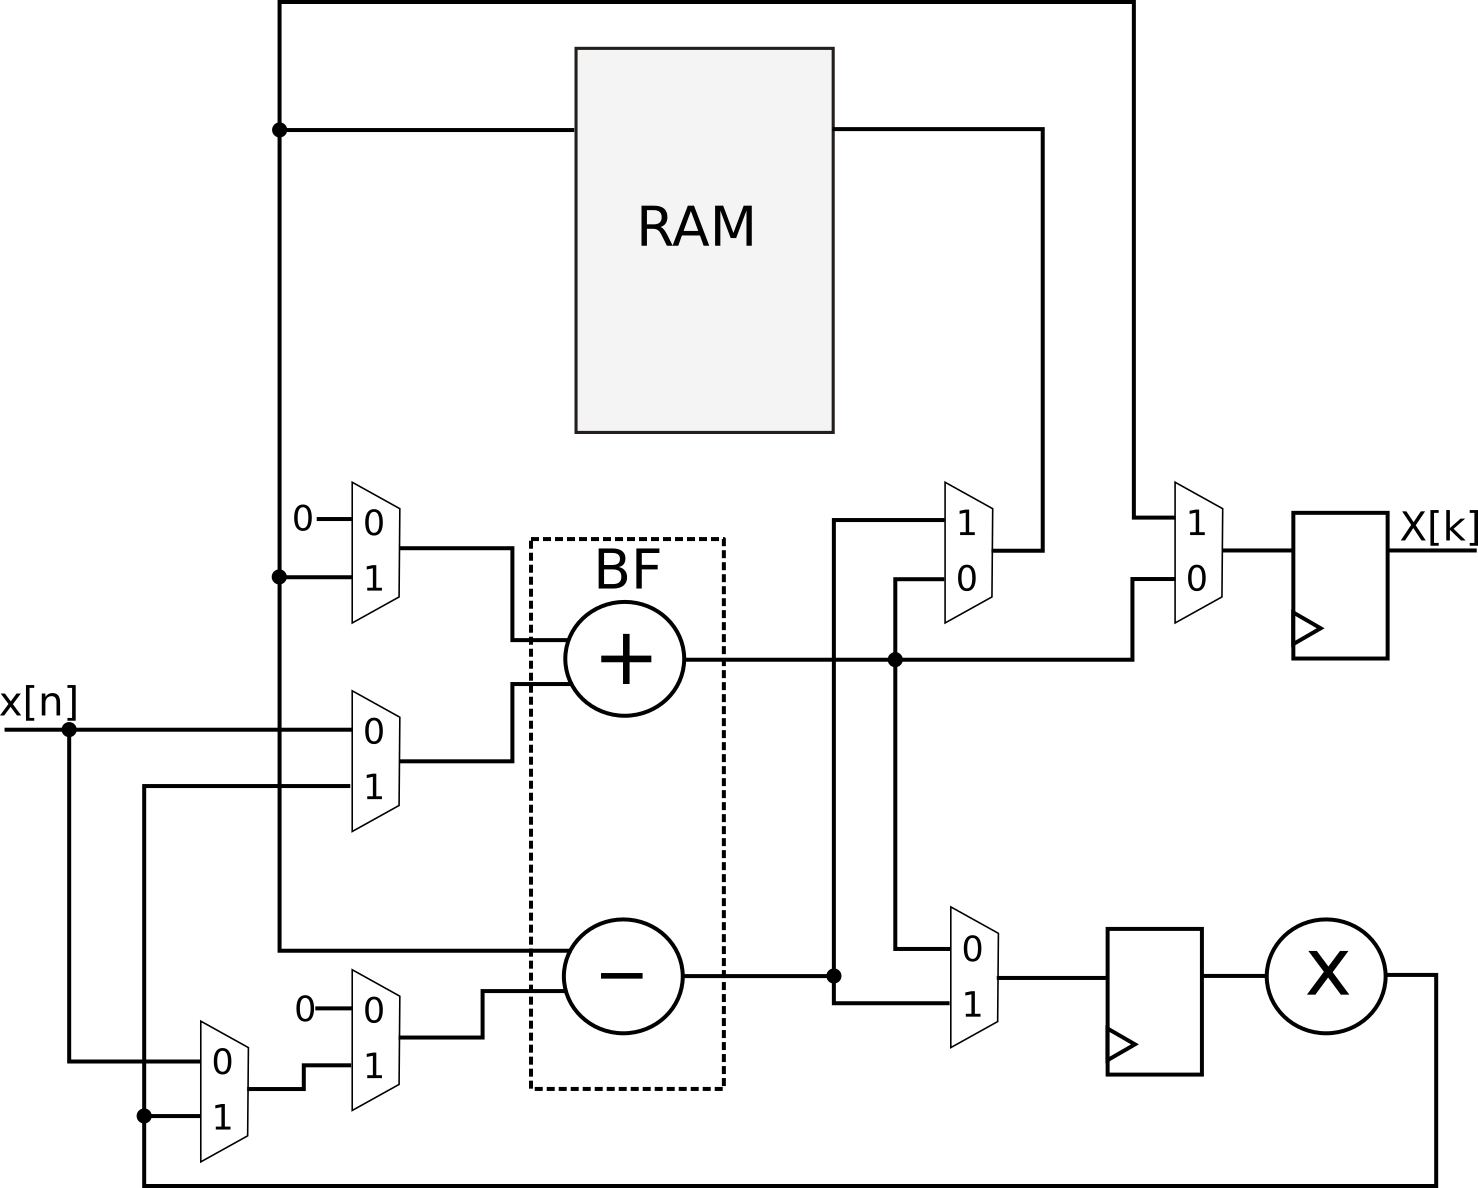
\includegraphics[scale=0.27]{./figures/datapath.png}
%         \end{center}
%       \end{column}
%       }
%       \uncover<4->{
%       \begin{column}{.5\textwidth}
%         \begin{center}
%           \advance\leftskip-0.2cm
%           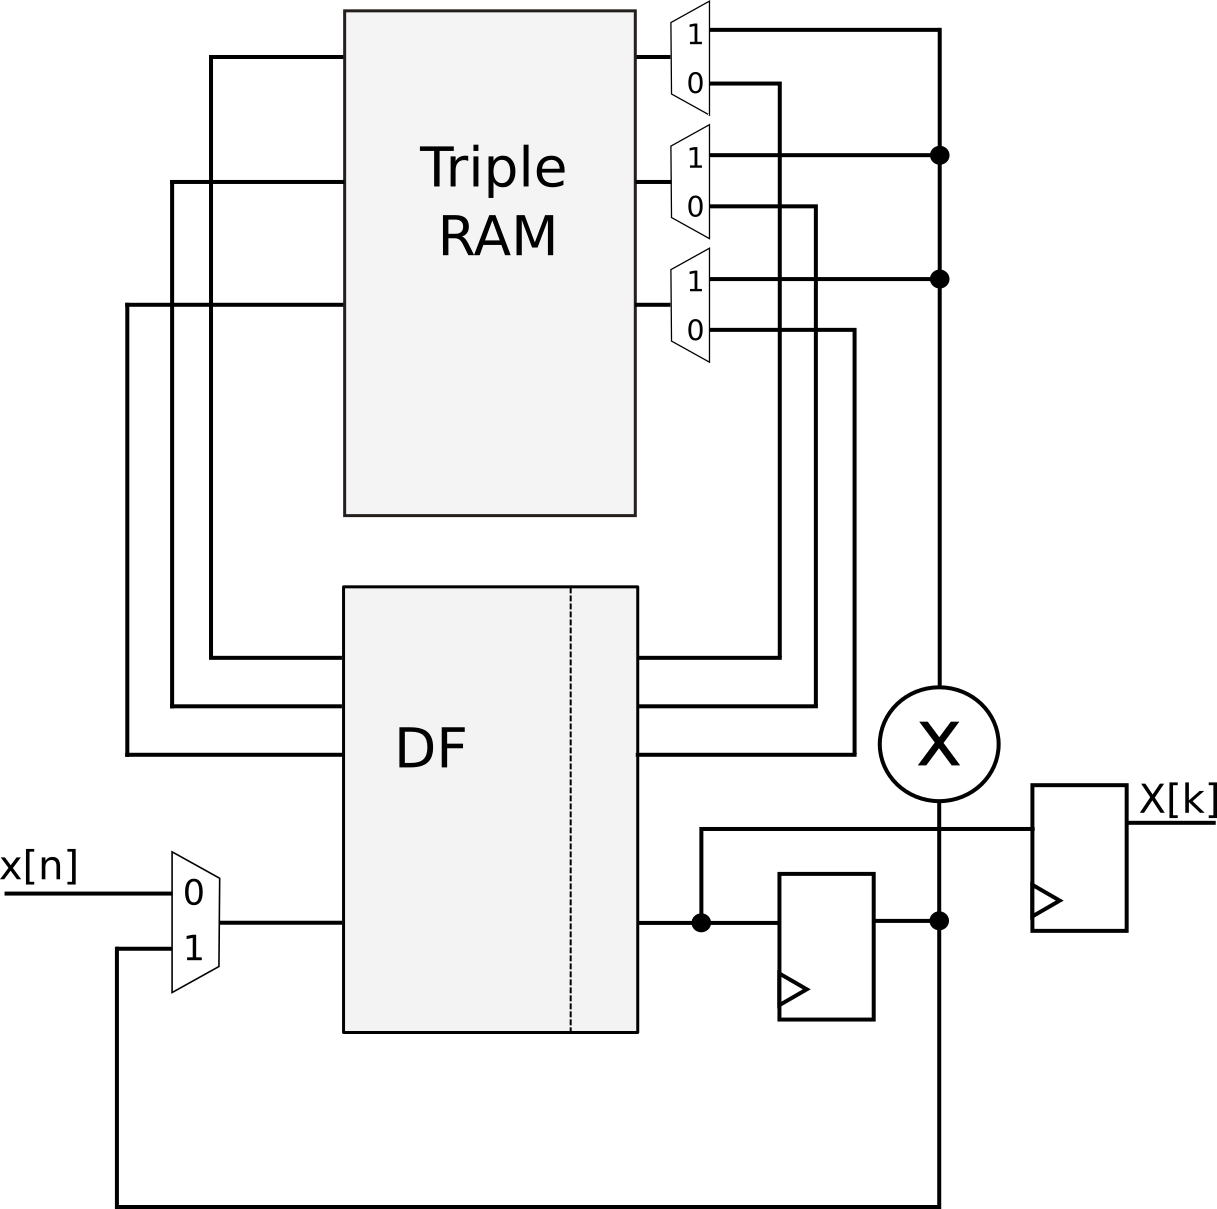
\includegraphics[scale=0.27]{./figures/datapathR4.png}
%         \end{center}
%       \end{column}
%       }
%   \end{columns}
%       
% \end{frame}
% 
% \begin{frame}{Datapath Radix-2}  
% 
%   \only<1-1>{
%   Etapa inicial
%   \begin{columns}[T]
%     \begin{column}{.5\textwidth}
%       \begin{center}
%         \advance\leftskip-0.2cm
%         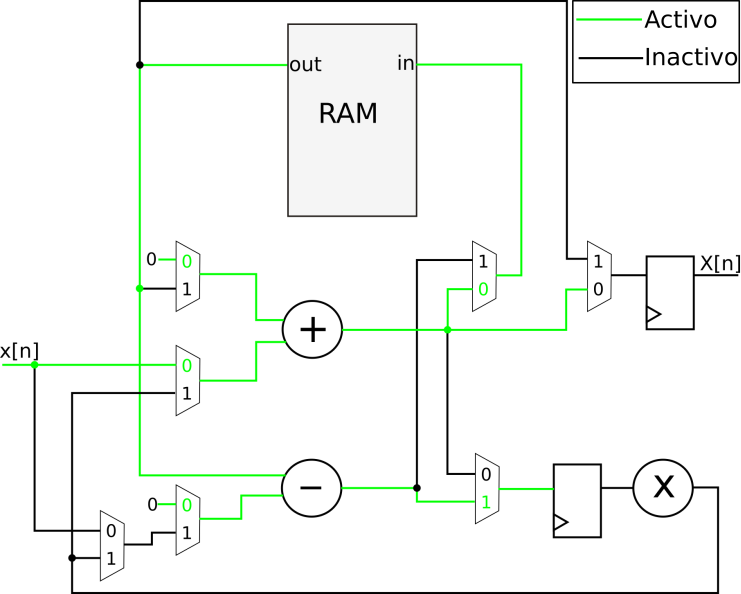
\includegraphics[scale=0.20]{./figures/datapath_mem1.png}
%       \end{center}
%     \end{column}
%     
%     \begin{column}{.5\textwidth}
%       \begin{center}
%         \advance\leftskip-0.2cm
%         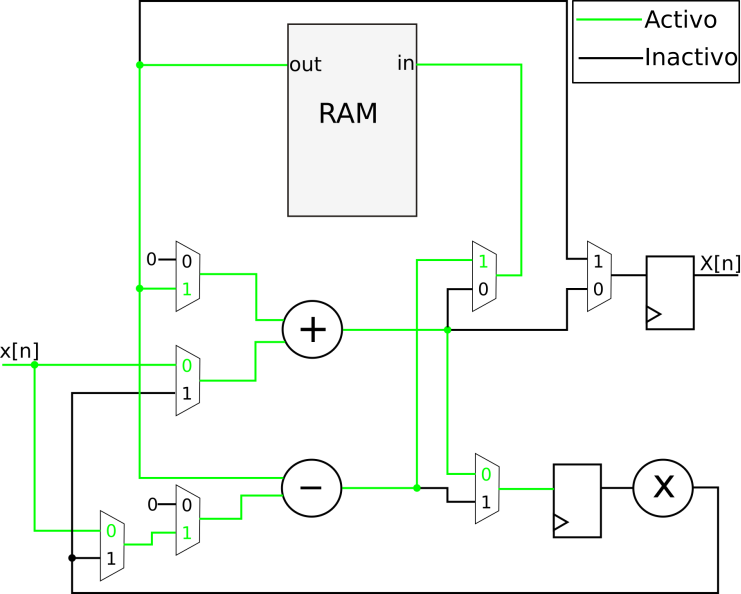
\includegraphics[scale=0.20]{./figures/datapath_but1.png}
%       \end{center}
%     \end{column}
%   \end{columns}
%   }
%   
%   \only<2-2>{
%   Etapas intermedias
%   \begin{columns}[T]
%     \begin{column}{.5\textwidth}
%       \begin{center}
%         \advance\leftskip-0.2cm
%         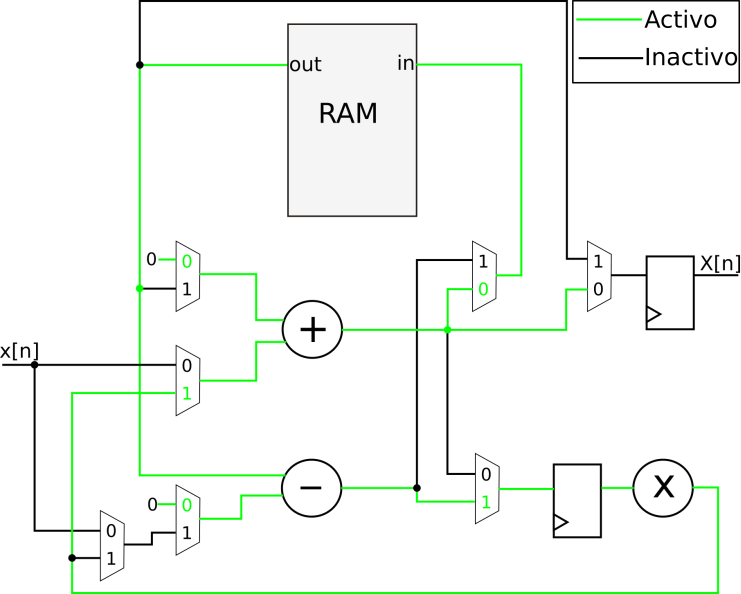
\includegraphics[scale=0.20]{./figures/datapath_memint.png}
%       \end{center}
%     \end{column}
%     
%     \begin{column}{.5\textwidth}
%       \begin{center}
%         \advance\leftskip-0.2cm
%         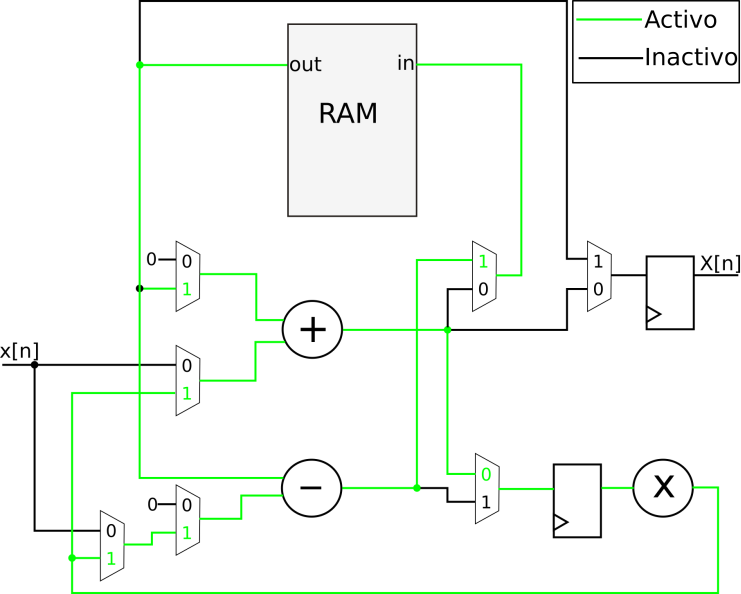
\includegraphics[scale=0.20]{./figures/datapath_butint.png}
%       \end{center}
%     \end{column}
%   \end{columns}
%   }
%   
%   \only<3-3>{
%   Etapa final
%   \begin{columns}[T]
%     \begin{column}{.5\textwidth}
%       \begin{center}
%         \advance\leftskip-0.2cm
%         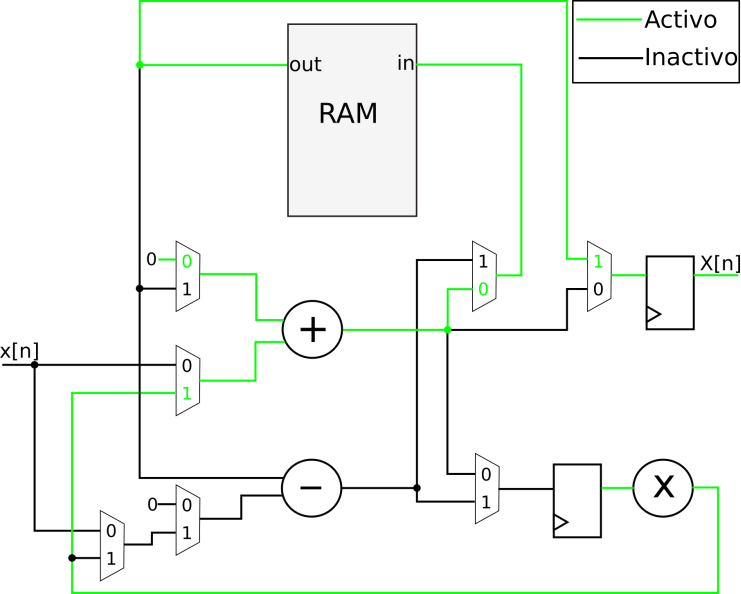
\includegraphics[scale=0.20]{./figures/datapath_memf.png}
%       \end{center}
%     \end{column}
%     
%     \begin{column}{.5\textwidth}
%       \begin{center}
%         \advance\leftskip-0.2cm
%         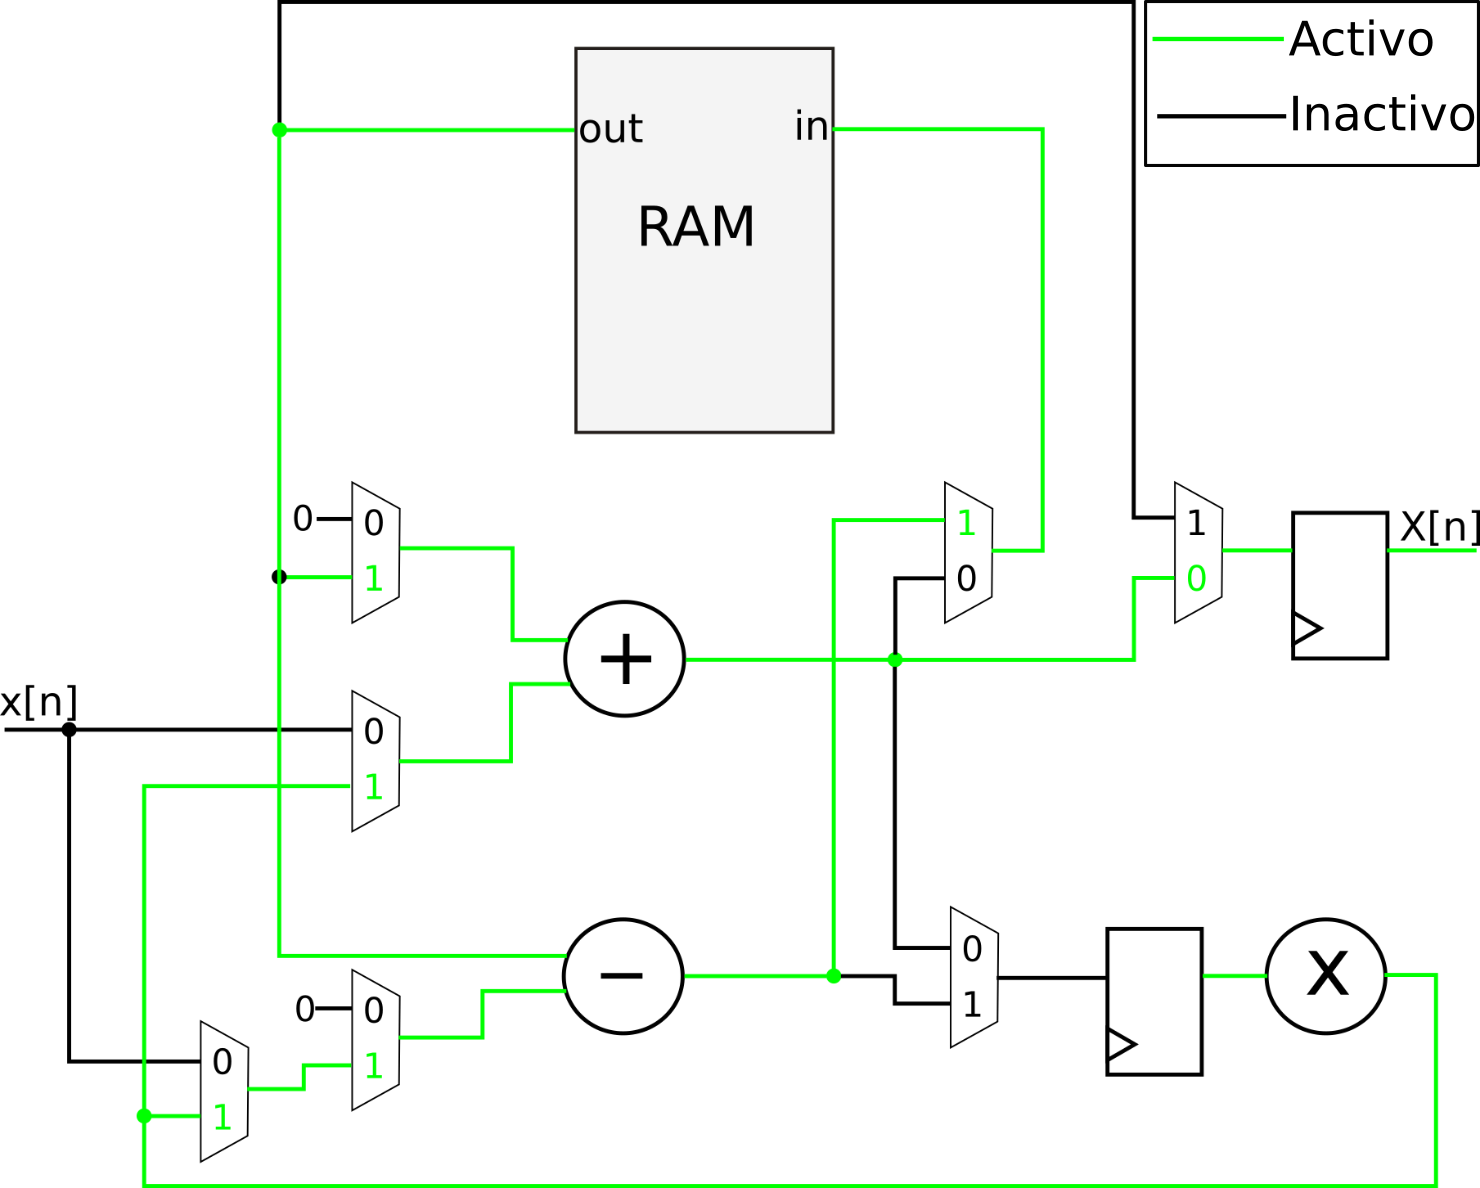
\includegraphics[scale=0.25]{./figures/datapath_butf.png}
%       \end{center}
%     \end{column}
%   \end{columns}
%   }
%   
% \end{frame}
% 
% \begin{frame}{Datapath Radix-4}
%   \only<1-1>{
%   Etapa inicial
%   \begin{columns}[T]
%     \begin{column}{.5\textwidth}
%       \begin{center}
%         \advance\leftskip-0.2cm
%         \includegraphics[scale=0.28]{./figures/datapathR4_mem_ini.png}
%       \end{center}
%     \end{column}
%     
%     \begin{column}{.5\textwidth}
%       \begin{center}
%         \advance\leftskip-0.2cm
%         \includegraphics[scale=0.28]{./figures/datapathR4_arit_ini.png}
%       \end{center}
%     \end{column}
%   \end{columns}
%   }
%   
%   \only<2-2>{
%   Etapas intermedias
%   \begin{columns}[T]
%     \begin{column}{.5\textwidth}
%       \begin{center}
%         \advance\leftskip-0.2cm
%         \includegraphics[scale=0.28]{./figures/datapathR4_mem_int.png}
%       \end{center}
%     \end{column}
%     
%     \begin{column}{.5\textwidth}
%       \begin{center}
%         \advance\leftskip-0.2cm
%         \includegraphics[scale=0.28]{./figures/datapathR4_arit_int.png}
%       \end{center}
%     \end{column}
%   \end{columns}
%   }
%   
%   \only<3-3>{
%   Etapa final
%   \begin{columns}[T]
%     \begin{column}{.5\textwidth}
%       \begin{center}
%         \advance\leftskip-0.2cm
%         \includegraphics[scale=0.28]{./figures/datapathR4_mem_fin.png}
%       \end{center}
%     \end{column}
%     
%     \begin{column}{.5\textwidth}
%       \begin{center}
%         \advance\leftskip-0.2cm
%         \includegraphics[scale=0.28]{./figures/datapathR4_arit_fin.png}
%       \end{center}
%     \end{column}
%   \end{columns}
%   }
%   
% \end{frame}
% 
% \subsection{Escalamiento}
% 
% \begin{frame}{Unidad de escalamiento}
%   \begin{itemize}
%     \item<1-> Hay riesgo de \textit{overflow}
%     \item<2-> 1 bit por etapa
%     \item<3-> División por 2
%     \begin{itemize}
%       \item<4-> Truncamiento
%       \item<5-> Redondeo
%     \end{itemize} 
%     \item<6-> Activación dinámica y diferenciada por etapa
%   \end{itemize}
%   
%   \uncover<7->{
%   \begin{center}
%     \advance\leftskip-0.2cm
%     \includegraphics[scale=0.42]{./figures/escBlocks.png}
%   \end{center}
%   }
%   
% \end{frame}
% 
% \subsection{Unidad de Control}
% 
% \begin{frame}{Unidad de Control - Descripción}
%   \begin{itemize}
% %     \item<1-> La unidad de control debe controlar el funcionamiento de la arquitectura
% %     \begin{itemize}
% %       \item<2-> Configuración del datapath
% %       \item<3-> Control de la memoria
% %       \item<4-> Generación de los twiddle factors
% %       \item<5-> Control del escalamiento para cada etapa
% %     \end{itemize}
%     \item<1-> El control se realiza mediante dos contadores
%     \begin{itemize}
%       \item<2-> Un contador de etapas, \textit{stg\_ctr}
%       \item<3-> Un contador de puntos, \textit{ptr\_ctr}
%     \end{itemize}  
%     \item<4-> El tipo de operación se determina analizando una posición del contador de
%     puntos 
%     \uncover<5-7>{
%     \begin{columns}[T]
%       \begin{column}{.5\textwidth}
% 	    \begin{center}
% 	      \advance\leftskip-0.2cm
% 	      \includegraphics[scale=0.22]{./figures/r2conts.png}
% 	    \end{center}
% 	    \begin{columns}[T]
% 	      \begin{column}{.2\textwidth}
% 	      
% 	      \end{column}
%           \begin{column}{.8\textwidth}
% 	        \begin{itemize}
% 	          \item<6-> `0': operación en memoria
% 	          \item<6-> `1': operación aritmética
% 	        \end{itemize}
% 	      \end{column}
% 	      \begin{column}{.1\textwidth}
% 	      
% 	      \end{column}
% 	    \end{columns}
% 	  \end{column}
% 	  
% 	  \begin{column}{.5\textwidth}
% 	    \begin{center}
%           \advance\leftskip-0.2cm
%           \includegraphics[scale=0.22]{./figures/r4conts.png}
%         \end{center}
%         \begin{columns}[T]
% 	      \begin{column}{.2\textwidth}
% 	      
% 	      \end{column}
%           \begin{column}{.8\textwidth}
%           \begin{itemize}
%             \item<7-> `00': operación a memoria A
%             \item<7-> `01': operación a memoria B
%             \item<7-> `10': operación a memoria C
%             \item<7-> `11': operación aritmética
%           \end{itemize}
%           \end{column}
% 	      \begin{column}{.1\textwidth}
% 	      
% 	      \end{column}
% 	    \end{columns}
% 	  \end{column}
%     \end{columns}
%     }
%  
% %     \item<6-> La memoria se direcciona con el contador de puntos
% %     \item<7-> El ángulo correspondiente al twiddle factor se genera en base a ambos contadores
%   \end{itemize}
% \end{frame}
% 
% \begin{frame}{Unidad de Control - Máquinas de estado}
%   
%   \begin{itemize}
%     \item<1-> La unidad de control funciona en base a dos máquinas de estados
%     \begin{itemize}
%       \Fontitit
%       \item<2-> Una máquina de estados principal. Inicialización y reset.
%       \item<4-> Una máquina de estados operativa. Configuración del datapath.
%     \end{itemize}
%   \end{itemize}
%   
%   \begin{columns}[T]
%     \uncover<3-5>{
%       \begin{column}{.4\textwidth}
%         \begin{center}
%           \advance\leftskip-0.2cm
%           \includegraphics[scale=0.35]{./figures/SMr2gen.png}
%         \end{center}
%       \end{column}
%     }
%     
%     \uncover<5-5>{
%       \begin{column}{.6\textwidth}
%         \begin{center}
%           \advance\leftskip-0.2cm
%           \includegraphics[scale=0.19]{./figures/SMr2op.png}
%         \end{center}    
%       \end{column}
%     }
%   \end{columns}
% \end{frame}
% 
% \subsection{Diseño final}
% 
% \begin{frame}{Diseño final de la arquitectura radix-2}
%   \begin{center}
%     \advance\leftskip-0.2cm
%     \includegraphics[scale=0.4]{./figures/datapathMem.png}
%   \end{center}
% \end{frame}
% 
% \begin{frame}{Diseño final de la arquitectura radix-4}
%   \begin{center}
%     \advance\leftskip-0.2cm
%     \includegraphics[scale=0.4]{./figures/datapathR4control.png}
%   \end{center}
% \end{frame}
% 
% 
% \subsection{Interfaces de las arquitecturas}
% \begin{frame}{}%{Interfaces de las arquitecturas}
%   \begin{center}
%     \advance\leftskip-0.2cm
%     \includegraphics[scale=0.5]{./figures/arcInterf.png}
%   \end{center}
% \end{frame}
\section{Caracterizaci�n y tests}

\begin{frame}
\begin{center}
\Huge CARACTERIZACI�N Y PRUEBAS
\end{center}
\end{frame}

\begin{frame}{Listado de pruebas}
  \begin{itemize}
	\item<1-> Transformaci�n de se�ales patr�n
	\item<2-> Medici�n del error
	\item<3-> Medici�n de la THD
	\item<4-> Efecto del escalamiento
	\item<5-> Medici�n de los recursos necesarios 
    \item<6-> Comparaci�n con core FFT abierto para modulaci�n OFDM/ISDB-T
  \end{itemize}
\end{frame}

% \subsection{Se�ales Patr�n}
% 
% \begin{frame}{Se�ales patr�n}
%   \uncover<1->{
%   \begin{itemize}
%     \item<1-> Se realizaron pruebas utilizando como entrada deltas en diferentes compoenentes y se
%     analiz� su salida. Por ejemplo:
%     \begin{itemize}
%       \item<2-> Una delta en posici�n `0'
%       \item<3-> Una delta en posici�n `6'
%     \end{itemize}
%   \end{itemize}
%   }
%   \uncover<2->{
%     \alt<2>{
%       \begin{center}
%         \advance\leftskip-0.2cm
%         \includegraphics[scale=0.3]{./figures/r2_delta0_16_4096_mul.png}
%       \end{center}
%     }{
%       \begin{center}
%         \advance\leftskip-0.2cm
%         \includegraphics[scale=0.3]{./figures/r2_delta7_16_4096_mul.png}
%       \end{center}
%     }
%   }
% \end{frame}

\subsection{Medici�n del error}
\begin{frame}{Medici�n del error}%{Métricas de error}
%   \only<1-8>{
%   \begin{itemize}
%     \item<1-> Las métricas utilizadas para estimar el error fueron
%     \begin{itemize}
%       \item<2-> $E_\infty = MAX\left(\frac{ X_o[n] - X_{dut}[n]}{X_o[n]}\right)$
%       \item<3-> $E_2 = \left\Vert\frac{X_o[n] - X_{dut}[n]}{X_o[n]}\right\Vert_2$
%     \end{itemize}
%     \item<4-> Dado que el sistema es no lineal se realizaron 1024 simulaciones
%     \begin{itemize}
%       \item<5-> Se creó una entrada aleatoria para cada simulación
%       \item<6-> Se calculó el error en cada simulación y luego se promedió
%       \item<7-> Se realizó para cada arquitectura
%       \item<8-> Se utilizó el cálculo de FFT de la señal de entrada en Matlab como referencia para
%       el cálculo de error
%     \end{itemize}
%     \item<9-> Se contrastó con el error de una arquitectura de cómputo de FFT de terceros: KISS
%       FFT en C++
%   \end{itemize}
%   }
  
%  \only<9>{
    \begin{columns}[T]
      \begin{column}{.44\textwidth}
        \begin{center}
          \advance\leftskip-0.2cm
          \includegraphics[scale=0.3]{./figures/error_sim.png}
        \end{center}
      \end{column}
      
      \begin{column}{.56\textwidth}
        \begin{center}
          \advance\leftskip-0.2cm
          \includegraphics[scale=0.3]{./figures/norm1_1024_12.png}
        \end{center}
        
        \begin{center}
          \advance\leftskip-0.2cm
          \includegraphics[scale=0.3]{./figures/norm1_r2_16_4096_mul.png}
          %\includegraphics[scale=0.2]{./figures/norm2_1024_12.png}
        \end{center}
        
%         \begin{center}
%           \advance\leftskip-0.2cm
%           \includegraphics[scale=0.3]{./figures/norm2_1024_12.png}
%         \end{center}
      \end{column}
    \end{columns}
%    }
\end{frame}

\begin{frame}{Resultados de la medici�n de error}

  \begin{columns}[T]
    \begin{column}{.2\textwidth}

    \end{column}
    \begin{column}{.8\textwidth}
	\begin{tabular}{l c c c c}
		& \textbf{1024, 12} & \textbf{1024, 16} & \textbf{4096, 12} & \textbf{4096, 16}\\ \hline 
		\textbf{R-2, cordic} & $0.092$ & $0.006$ & $0.099$ & $0.008 $\\
		\textbf{R-2, Mult.} & $0.232$ & $0.003$ & $0.340$ & $0.108$\\
		\textbf{R-4, cordic} & $0.077$ & $0.003$ & $0.074$ & $0.007$\\
		\textbf{R-4, Mult.} & $0.224$ & $0.002$ & $0.334$ & $0.105$\\
		\textbf{Kiss FFT} & $ $ & $0.017$ & $ $ & $0.035$\\
		\textbf{Xilinx FFT v7.1} & $0.0007$ & $0.0001$ & $0.0008$ & $0.0004$\\ \hline
	\end{tabular}\\
	\end{column}
	
	\begin{column}{.2\textwidth}
	
	\end{column}

  \end{columns}
	
% 	Resultados para $E_2$
% 	\begin{tabular}{l c c c c }
% 		 & \textbf{1024, 12} & \textbf{1024, 16} & \textbf{4096, 12} & \textbf{4096, 16}\\ \hline 
% 		\textbf{R-2, cordic} & $0.095$ & $0.007$ & $0.116$ & $0.053$\\
% 		\textbf{R-2, Mult.} & $0.257$ & $0.004$ & $0.356$ & $0.131$\\
% 		\textbf{R-4, cordic} & $0.084$ & $0.002$ & $0.094$ & $0.027$\\
% 		\textbf{R-4, Mult.} & $0.258$ & $0.003$ & $0.358$ & $0.126$\\ 
% 		\textbf{Kiss FFT} & $ $ & $0.017$ & $ $ & $0.035$\\\hline
% 	\end{tabular}

\end{frame}

\subsection{Medici�n de la THD}
% \begin{frame}{Medici�n de la THD}
% %   \only<1-5>{
% %   \begin{itemize}
% %     \item<1-> Las arquitecturas se comportan como sistemas no lineales
% %     \item<2-> Para medir completamente la THD no alcanza con medir para algunas frecuencias
% %     \item<3-> Se midió la THD para entradas delta en cada una de las componentes para cada
% %     arquitectura
% %     \item<4-> Se tomó la salida de cada simulación y se calculó la THD mediante Matlab.
% %     \item<5-> Se contrastó con la THD de la arquitectura Kiss FFT en C++.
% %   \end{itemize}
% %   }
%   
% %  \only<6>{
%     \begin{center}
%       \advance\leftskip-0.2cm
%       \includegraphics[scale=0.27]{./figures/thd_sim.png}
%     \end{center}
% %  }  
% \end{frame}

\begin{frame}{Medici�n de la THD}
  \begin{columns}[T]
    \begin{column}{.5\textwidth}
      %\only<1-1>{
        \begin{center}
	      %\advance\leftskip-0.2cm
	      \includegraphics[scale=0.17]{./figures/thd_r2_4096_16_cor.png}\\
          Radix-2, Cordic, 16 bits
        \end{center}
       % }
	    
	    
	    \begin{center}
	      %\advance\leftskip-0.2cm
	      \includegraphics[scale=0.17]{./figures/thd_r4_1024_16_mul.png}\\
	      Radix-4, Mult., 16 bits
	    \end{center}
	    
	  %\only<2-2>{  
% 	    \begin{center}
% 	      %\advance\leftskip-0.2cm
% 	      \includegraphics[scale=0.15]{./figures/thd_kiss_4096_16.png}\\
% 	      Kiss FFT. C++. 16 bits
% 	    \end{center}
	  %}
	    
    \end{column}
    
    \begin{column}{.5\textwidth}
%       \only<1-1>{
%         \begin{center}
% 	      %\advance\leftskip-0.2cm
% 	      \includegraphics[scale=0.15]{./figures/thd_r2_4096_16_mul.png}\\
% 	      Radix-2, Mult., 16 bits
% 	    \end{center}
% 	    }
	    
	    
	    \begin{center}
	      %\advance\leftskip-0.2cm
% 	      \includegraphics[scale=0.15]{./figures/thd_r4_1024_16_mul.png}\\
% 	      Radix-4, Mult., 16 bits
	       \includegraphics[scale=0.17]{./figures/thd_kiss_4096_16.png}\\
	      Kiss FFT. C++. 16 bits
	    \end{center}
	    
%	  \only<2-2>{  
	    \begin{center}
	      %\advance\leftskip-0.2cm
	      \includegraphics[scale=0.17]{./figures/thd_xilinx_r4_16_1024.png}\\
	      Xilinx LogiCORE FFT 7.1
	      %Matlab. Punto flotante 64 bits
	    \end{center}
%	  }
	    
    \end{column}
  \end{columns}
\end{frame}

% \begin{frame}{Análisis de la intermodulación}
% %   \begin{itemize}
% %     \item<1-> Se midió la THD para un tono determinado
% %     \item<2-> Se midió la THD para una señal que contiene el mismo tono y el tono inmediato
% %     anterior, y se comparó con la THD anterior
% %   \end{itemize}
% %   \uncover<3-4>{
% %   \begin{columns}[T]
% %     \begin{column}{.5\textwidth}
% % \begin{itemize}
% %   \item<1-> Señal que produce overflow 
%       \begin{center}
%         \advance\leftskip-0.2cm
% 	    \includegraphics[scale=0.22]{./figures/thd_r2_4096_16_cor_450_451.png}\\
% 	    Rotador Cordic.
% 	  \end{center}
% % 	\end{column}
% 	
% % 	\begin{column}{.5\textwidth}
% %   \item<2-> Señal con produce overflow
% 	  \begin{center}
% 	    \advance\leftskip-0.2cm
% 	    \includegraphics[scale=0.22]{./figures/thd_r2_4096_16_mul_450_451.png}\\
% 	    Multiplicador complejo.
% 	  \end{center}
% % 	\end{column}
% %   \end{columns}
% %   }
% %   \begin{itemize}
% %     \item<4-4> Se observa que no hay efectos de intermodulación 
% %   \end{itemize}
% \end{frame}

% \subsection{Efecto del escalamiento}
% 
% \begin{frame}{}
%   \begin{itemize}
%     \item<1-> Ensayos de verificación
%     \begin{itemize}
%       \Fontitit
%       \item<1-> Transformación de señales patrón
%     \end{itemize}
%     \item<1-> Ensayos de caracterización
%     \begin{itemize}
%       \Fontitit
%       \item<1-> Medición del error
%       \item<1-> Medición de la THD
%       \item<1-> \color<1->[rgb]{0,0.6,0}Efecto del escalamiento
%       \item<1-> Medición de los recursos necesarios 
%     \end{itemize}
%     \item<1-> Ensayos de validación
%     \begin{itemize}
%       \Fontitit
%       \item<1-> Implementación en FPGA
%     \end{itemize}
%   \end{itemize}
% \end{frame}
% 
% \begin{frame}{Efecto sobre la señal de salida}
%   \begin{itemize}
%     \item<1-> Provoca un escalamiento por $1/2$ por cada etapa donde se realiza escalamiento
%     \item<2-> Provoca una pérdida de información
%   \end{itemize}
%   
%   \uncover<3-3>{
%     \begin{center}
%       \advance\leftskip-0.2cm
%       \includegraphics[scale=0.32]{./figures/rand_r2_16_4096_mul_trunc_2.png}\\
%     \end{center}
%     }
% \end{frame}
% 
% \begin{frame}{Utilidad en caso de overflow}
%   \begin{itemize}
% %     \item<1-> Se utilizaron dos señales compuestas por una delta en una componente
% %     \item<2-> Una dentro del rango de funcionamiento seguro y una que provoca overflow
% %     \item<3-> Se simuló con escalamiento en cada etapa y se midió la THD en cada caso
% %   \end{itemize}
% %   
% %   \uncover<4-4>{
% %   \begin{columns}[T]
% %     \begin{column}{.5\textwidth}
%      \item<1-> Señal sin producir overflow
% 	  \begin{center}
% 		  \advance\leftskip-0.2cm
% 		  \includegraphics[scale=0.21]{./figures/r2_16_4096_mul_scale_thd_red.png}
% 		\end{center}
% %     \end{column}
% %     \begin{column}{.5\textwidth}
%       \item<2-> Señal que provoca overflow
% 		\begin{center}
% 		  \advance\leftskip-0.2cm
% 		  \includegraphics[scale=0.21]{./figures/r2_16_4096_mul_scale_thd_05_red.png}
% 		\end{center}
%     \end{itemize}
% % 	\end{column}
% %   \end{columns}
% %   }
% \end{frame}

\subsection{Recursos de Implementaci�n}
% \begin{frame}{Recursos de implementaci�n}
%     \begin{columns}[T]
%       \begin{column}{.53\textwidth}
%       \begin{itemize}
%         \item<1-> Uno de los requerimientos es la econom�a de recursos
%         \item<2-> FPGA XC5VLX110, de la familia Virtex-5 de Xilinx.
%         \item<3-> Se compar� con dos arquitecturas
%         \begin{itemize}
%           \item<4-> Radix-2 desenrrollada
%           \item<5-> Xilinx LogiCORE FFT 7.1
%         \end{itemize}
%       \end{itemize}
%       \end{column}
%       \begin{column}{.47\textwidth}
%         \centering
%         \begin{center}
% 		  \advance\leftskip-0.2cm
% 		  \includegraphics[scale=0.32]{./figures/virtex_chip.jpg}
% 		\end{center}
%       \end{column}
%     \end{columns}
% %   \end{itemize}
% \end{frame}

\begin{frame}{Tama�o de implementaci�n para 1024 puntos}
%  \uncover<3-3>{
%   \begin{columns}[T]
%     \begin{column}{.5\textwidth}

	  \begin{center}
		  %\advance\leftskip-0.2cm
		  \includegraphics[scale=0.72]{./figures/sizecomp1024.png}\\
		  
		\end{center}
%     \end{column}
\end{frame}

\begin{frame}{Tama�o de implementaci�n para 4096 puntos}
%     \begin{column}{.5\textwidth}
		\begin{center}
		  %\advance\leftskip-0.2cm
		  \includegraphics[scale=0.72]{./figures/sizecomp4096.png}\\
		\end{center}
% 	\end{column}
%   \end{columns}
%   }
\end{frame}

% \subsection{Implementaci�n en hardware}
% 
% \begin{frame}{}%{Listado de pruebas}
%   \Fontit
%   \begin{itemize}
%     \item<1-> Ensayos de verificación
%     \begin{itemize}
%       \Fontitit
%       \item<1-> Transformación de señales patrón
%     \end{itemize}
%     \item<1-> Ensayos de caracterización
%     \begin{itemize}
%       \Fontitit
%       \item<1-> Medición del error
%       \item<1-> Medición de la THD
%       \item<1-> Efecto del escalamiento
%       \item<1-> Medición de los recursos necesarios 
%     \end{itemize}
%     \item<1-> Ensayos de validación
%     \begin{itemize}
%       \Fontitit
%       \item<1-> \color<1->[rgb]{0,0.6,0}Implementación en FPGA
%     \end{itemize}
%   \end{itemize}
% \end{frame}
% 
% \begin{frame}{Validación en hardware}
%   \only<1-2,4-5>{
%     
%       \begin{columns}[T]
%         \begin{column}{.5\textwidth}
%           \begin{itemize}
%             \item<1-> Se un placa de desarrollo Avnet, con una FPGA XC5VLX110
%             \item<2-> Se implementó adicionalmente una unidad de comuniación UART y una memoria
%        auxiliar.
%           \end{itemize}
%         \end{column}
%         \begin{column}{.5\textwidth}
%           \centering
%           \begin{center}
% 		    \advance\leftskip-0.2cm
% 		    \includegraphics[scale=0.48]{./figures/virtex_board.jpg}
% 		  \end{center}
%         \end{column}
%       \end{columns}
%       \begin{itemize}
%         \item<4-> Se utilizaron como entrada las señales patrón ya utilizadas previamente, y señales
%         aleatorias para las que se calculó el error.
%         \item<5-> Los resultados de las corridas fueron similares al obtenido previamente en las
%         simulaciones
%       \end{itemize}
%   }
%   
%   \only<3-3>{
%     \begin{center}
% 	  \advance\leftskip-0.2cm
% 	  \includegraphics[scale=0.38]{./figures/hw_tb.png}\\
% 	\end{center}
%   }
% \end{frame}

\subsection{Comparaci�n con IP Core FFT abierto}
\begin{frame}{Comparaci�n con IP Core FFT abierto}
	\begin{itemize}
	  \item<1-> IP Core abierto para modulaci�n/demodulaci�n OFDM para ISDB-T (Melo, R., Salom\'on, F., Valinoti, B., (2016) ``IP core FFT configurable en Runtime'')
	  \item<2-> Comparaci�n con la versi�n b�sica del IP Core, 8K muestras, 16 bits 
	\end{itemize}
	
	\begin{columns}[T]
    \begin{column}{.2\textwidth}

    \end{column}
    \begin{column}{.8\textwidth}
		\uncover<3->{
			\begin{tabular}{l c c }
			 & \textbf{Iterative radix-2} & \textbf{Reference core}\\ \hline 
			\textbf{FF} & $533$ & $1334$\\
			\textbf{LUT} & $3046$ & $4133$\\
			\textbf{BRAM} & $62$ & $62$\\
			\textbf{MUL} & $ $ & $48$\\ 
			\textbf{MHz} & $107$ & $61$\\ \hline
			\end{tabular}
		}
	\end{column}
	\begin{column}{.2\textwidth}

    \end{column}
    \end{columns}

\end{frame}


\section{Conclusiones y trabajos futuros}

\begin{frame}
\begin{center}
\Huge CONCLUSIONES Y TRABAJOS FUTUROS
\end{center}
\end{frame}

\subsection{Conclusiones}
\begin{frame}{Conclusiones}

\begin{itemize}
%   \item<1-> Se diseñaron e implementaron dos arquitecturas para el cómputo de la FFT
  \item<1-> Las arquitecturas implementadas cumplen con el requerimiento de la economía de recursos
%   \item<3-> Se desarrollaron dos módulos para el producto por los twiddle factors
  \item<2-> Se realizaron ensayos de verificación y caracterización
  \begin{itemize}
    \item<3-> Error dentro de los parámetros aceptables
    \item<4-> Baja distorsión
    \item<5-> Muy baja demanda de recursos
  \end{itemize} 
  \item<6-> Del resultado de los ensayos se concluye 
  \begin{itemize}
    \item<7-> Se cumplió con los requerimientos de desempeño
    \item<8-> Se cumplió con los requerimientos de flexibilidad y escalabilidad
  \end{itemize}
  \item<9-> Las arquitecturas son aptas para su utilización en la modulación de un sistema OFDM       
\end{itemize}

\end{frame}

\subsection{Trabajos futuros}
\begin{frame}{Trabajos Futuros}
  \begin{itemize}
	\only<1-3>{
	\item<1-> Estudiar posibles implementaciones de algoritmos de \textit{dithering} para
	reducir el ruido generado en las arquitecturas.
	\item<2-> Modificar el módulo de rotación Cordic agregando un pipeline que permita aumentar la
	velocidad de \textit{clock} de las arquitecturas, sin agregar ciclos de \textit{clock} extra al
	cómputo total de la FFT.
	\item<3-> Modificar el multiplicador complejo agrandando el tamaño de palabra de los factores de
	multiplicación de los \textit{twiddle factors} y/o optimizarlo para la utilización de los bloques
	de procesamiento digital de los dispositivos FPGA.
	}
	\only<4-5>{
	\item<4-> Modificar el hardware para que el tamaño de palabra del ángulo de rotación sea
	independiente del tamaño de palabra de las señales.
	\item<5-> Estudiar la posibilidad de modificar las arquitecturas de forma de poder modificar la
	cantidad de puntos de la FFT en forma dinámica.
	}
 \end{itemize}
\end{frame}

\begin{frame}
%\frametitle{A first slide}

\begin{center}
\Huge ¿PREGUNTAS?
\end{center}

\end{frame}

\begin{frame}
%\frametitle{A first slide}

\begin{center}
\Huge MUCHAS GRACIAS!
\end{center}

\end{frame}

\begin{frame}
%\frametitle{A first slide}

\begin{center}
\Huge FIN!
\end{center}

\end{frame}

\end{document}
